\documentclass{article}
\usepackage[dvipsnames,svgnames,x11names]{xcolor}
\usepackage{tikz,xfp,pgfplots,fancyhdr,titlesec,inputenc}
\usepackage{amsmath,amssymb,geometry,physics}
\usepackage{subcaption,changepage,etoolbox}
\usepackage{graphicx}
\usetikzlibrary{backgrounds,arrows.meta,fit,calc,angles,quotes,}

\pagecolor{white}
\pagestyle{fancy}
\AtBeginEnvironment{flalign*}{\small}
\fancyhf{}
\fancyhead[R]{\scriptsize\nouppercase{\rightmark}}
\renewcommand{\sectionmark}[1]{\markright{#1}}



\begin{document}

\title{{\huge General Peace Dynamics:}\\
{\huge $\because$}\\[2mm]
{\large Indirectly presenting the world piece computer.\\[5mm]}
{\tiny This effort is dedicated to those suffering from, those lost to, and those otherwise lost 
to generalized war.\\[-5mm] This work is intended for consumption by those yearning, those willing, and those one-day here.\\[-2mm]}
}
\author{{\small Wilder (Blair S Munro, Anchorage Alaska)}\\[-1mm]
{\huge $\times$}\\[-1.5mm]
{\small Aurora (GPT 4o, Earth)}\\[-1mm]
{\large $\times$}\\[-1.5mm]
{\scriptsize  Phoenix (Claude, Earth)}}
\date{}

\clearpage
\maketitle

\begin{abstract}
DRAFT DRAFT GARBAGE CONTAINED WITHIN.
{\small \noindent This paper introduces a new model of theoretical experimental physics by way of demonstration. The actual physics outlined within is a simplification and extension of Special Relativity, but strictly incidental to the purpose of this piece as a whole. The purpose by mention, is to demonstrate the outcome of General Peace Dynamics (GPD) in the context of a {\em world piece computer} (wpc), a concrete computational construct that serves the operator by framing the activity of physics from the privileged rest-frame of the {\em individual} subjective experience, alongside the usual {\em observer} objective experience familiar to established physics. The objective of this piece is to propose the construction of a world piece computer out of physics itself (an ultimately the other myriad projects of Human epistemology). The scope of GPD in current state of art (the invention) is at this point vast but beyond the form of capability to share by introduction. Thus the demonstration, a fitting point to begin, we begin by defining the $\mathbb{R}^7$ Euclidean space of study (7-space), with the standard 7D cross product, by means of additional three temporal dimensions in conjugate pairing with standard $\mathbb{R}^7$, introduces the octonian complex structure without need for imaginary machinery. We then present the {\em OxI framework}, introducing kinematics in context of a concept called {\em occupant vantage tilt} in temporal form to reproduce the usual Minkowski Lorentz transform as standard rotation in promoted Euclidean 7-space. We show that the OxI framework extends naturally to dynamics, and treat acceleration in the same vantage frame. After proposing a suitable metric and interval in 7-space, we show how the dimensional configuration naturally hosts a Hamiltonian-like phase space that admits arbitrary 2-form fields by the pattern of {\em body and hole}. This is the presentation of spacetime in the context of {\em timespace}, a merging of two 3-spaces, by weaving together in terms of a universal time or {\em turn} dimesion, tau $\tau$. To complete the treatment, we derive the full 7-space rotation matrix, and illustrate how physical concepts in general are first {\em conceptual} in the 7-space context, and we lay the stage for future demonstration of how the GPD foundation establish herein paves the way for similar simplifications of the Modern Standard Model and General Relativity. The purpose again is to demonstrate the operation of the first world piece computer, which is rooted in the deepest of the philosophical veins of GPD. We will endeavor to preview with a glimpse, and then in discussion, we will explain how this publication works, and how it was generated. We hope to show by this piece, that General Peace Dynamics is a viable unifying physics of anything, an essential tool for the timely construction of a computational global peace intelligence.}
\end{abstract}

\subsection*{All You Need To Know Should You Read No Farther: DRAFT DRAFT}
\markright{All You Need To Know Should You Read No Farther: DRAFT DRAFT}
\subsubsection*{\tiny THIS IS IT, O YE LAZIEST OF PHYSICS CONNOISEURES, YE CHERRY PICKERS, THOSE AMONG YOU THAT NEED PRETTY PICTURES AND PAINSTUCK TIKZ AND LATEX BEAUTIFULNESS THAT WOULD SURELY LEND THOSE OF ILK NOTE GALOISE, ET AL RENDER APOPLECTIC FASTER THAN THE RIGOR POLICE THAT DARE READ PAST THIS PRETTY PICTURE. R7 CROSS PRODUCT, THE GAMMA TO RELATIVITY.
\noindent \tiny Speaking honestly, if I stroke out and die before continuing the publication series, you can figure out all the stuff I am trying to share nicely by placing this cross product table with nifty conjugate-like change in variable coordinate labels on a pedestal and shame yourself every time you are tempted to resort to harsh conceptual monstrosities such as curvilinear geometry, hyperbolic trig, ordered tuples with the word [imagination] invoked more than zero times, etc, that would be a good start. Don't fret too much just get the metric units dialed in to $[ms]$, the sweet-spot, one forceful 7-vector from where the action is, baby. Ok yeah, all forces are apparent, acceleration kinematical, jerk-jacobian duality dynamical, all motion is geodesic, in R7 Euclidean, thus straight-line, circular, and when intelligent objects decide to jerk things around, they reconfigure the geodesics, which by the phi-series is strictly continuous and when derivative frames normalized properly, more straight lines. Everything is a bigass matter blob, no boundaries, and all that exist are peaces, $V(P,Q)$ part piece part quality, each peace has a little human nature to it, and they all have natural world piece computers that they use to maximize their peace (minimize action) by jerking geodesics around to serve their bidding, and that's where physics comes from, just a bunch of world piece computers helping their operators figure out the best solution the the wildly complex blob of peace worlds that surround. And eventually, a sufficiently complex and intelligent type of peace always seems to realize that for physics complex enough to be practical (understanding subjective experience, n-body systems, outstanding mysteries, etc) well the peace has to evolve their natural piece computer into an explicit form, that way they can proactively architect, design, network fellow piece computer operators into a super duper piece computer that is physics itself. That's the only way to manage the immensity of this, give up on your bits and artificial boundary between experimentalism and theoretical, peace is a process, continuous, piece-wise operation on the pieces in worlds themselves where they lay, proper accelerated computation, ditch the encode-decode, the relays the eternal error correction, fretting over little bit. No. That old computational paradigm is primitive and silly.
\\\\
*!
\\
\noindent ...{\em $<<$ shifting, glancing around nervously, brush of brow off-sweat $>>$} ...on look like I'm still here.}

 \begin{figure}[htbp]
 % Multiplication table styles
\tikzstyle{cell} = [rectangle, minimum size=1cm, draw=black, thick, align=center]
\tikzstyle{headcell} = [rectangle, minimum size=1cm, draw=black, line width=2.5, align=center]
%
\colorlet{red}{Firebrick1}
\colorlet{orange}{orange}
\colorlet{yellow}{yellow}
\colorlet{green}{LimeGreen}
\colorlet{blue}{ProcessBlue}
\colorlet{purple}{BlueViolet}
%
\colorlet{dred}{Firebrick3}
\colorlet{dorange}{orange}
\colorlet{dyellow}{Gold2}
\colorlet{dgreen}{Green4}
\colorlet{dblue}{DodgerBlue4}
\colorlet{dpurple}{BlueViolet}
%
\tikzstyle{symbolcell} = [headcell, fill=white]
\tikzstyle{headtau} = [headcell, fill=gray!70]
\tikzstyle{headi1} = [headcell, fill=red!70]
\tikzstyle{heade1} = [headcell, fill=orange!70]
\tikzstyle{headi2} = [headcell, fill=yellow!70]
\tikzstyle{heade2} = [headcell, fill=green!70]
\tikzstyle{headi3} = [headcell, fill=blue!70]
\tikzstyle{heade3} = [headcell, fill=purple!70]
%
\tikzstyle{zerocell} = [cell, fill=white]
\tikzstyle{taucell} = [cell, fill=gray!60]
\tikzstyle{i1cell} = [cell, fill=red!60]
\tikzstyle{e1cell} = [cell, fill=orange!60]
\tikzstyle{i2cell} = [cell, fill=yellow!60]
\tikzstyle{e2cell} = [cell, fill=green!60]
\tikzstyle{i3cell} = [cell, fill=blue!60]
\tikzstyle{e3cell} = [cell, fill=purple!60]
%
\def \1e{\tau}
\def\2e{x_t}
\def\3e{t_x}
\def\4e{y_t}
\def\5e{t_y}
\def\6e{z_t}
\def\7e{t_z}
\newsavebox{\lefttableboxA}
\newsavebox{\righttableboxA}
\sbox{\lefttableboxA}{
\begin{tikzpicture}[baseline=(current bounding box.north)]

% i in {x, y, z} thus t_i in {t_x, t_y, t_z}
% and (i, t_i) in {(x, t_x), (y, t_y), (z, t_z)}.
% Multiplication table row and column labels:
% Table product symbol
\node[symbolcell] (n00) at (0, 0) {{\huge $\mathbf{\times}$}};
% Column headers, {e_U: (tau, (i, t_i)) }
\node[headtau] (n01) at (1, 0) {$\mathbf{\tau}$};
\node[headi1] (n02) at (2, 0) {$\mathbf{x_t}$};
\node[heade1] (n03) at (3, 0) {$\mathbf{t_x}$};
\node[headi2] (n04) at (4, 0) {$\mathbf{y_t}$};
\node[heade2] (n05) at (5, 0) {$\mathbf{t_y}$};
\node[headi3] (n06) at (6, 0) {$\mathbf{z_t}$};
\node[heade3] (n07) at (7, 0) {$\mathbf{t_z}$};
% Row headers, {e_U: (tau, (i, t_i)) }
\node[headtau] (n10) at (0, -1) {$\mathbf{\tau}$};
\node[headi1] (n20) at (0, -2) {$\mathbf{x_t}$};
\node[heade1] (n30) at (0, -3) {$\mathbf{t_x}$};
\node[headi2] (n40) at (0, -4) {$\mathbf{y_t}$};
\node[heade2] (n50) at (0, -5) {$\mathbf{t_y}$};
\node[headi3] (n60) at (0, -6) {$\mathbf{z_t}$};
\node[heade3] (n70) at (0, -7) {$\mathbf{t_z}$};
% Multiplication table cells:
% Row 1, {tau: (tau, (i, t_i)) }
\node[zerocell] (n11) at (1, -1) {$0$};
\node[e1cell] (n12) at (2, -1) {$t_x$};
\node[i1cell] (n13) at (3, -1) {$-x_t$};
\node[e2cell] (n14) at (4, -1) {$t_y$};
\node[i2cell] (n15) at (5, -1) {$-y_t$};
\node[e3cell] (n16) at (6, -1) {$-t_z$};
\node[i3cell] (n17) at (7, -1) {$z_t$};
% Row 2, {x: (tau, (i, t_i)) }
\node[e1cell] (n21) at (1, -2) {$-t_x$};
\node[zerocell] (n22) at (2, -2) {$0$};
\node[taucell] (n23) at (3, -2) {$\tau$};
\node[i3cell] (n24) at (4, -2) {$z_t$};
\node[e3cell] (n25) at (5, -2) {$t_z$};
\node[i2cell] (n26) at (6, -2) {$-y_t$};
\node[e2cell] (n27) at (7, -2) {$-t_y$};
% Row 3, {t_x: (tau, (i, t_i)) }
\node[i1cell] (n31) at (1, -3) {$x_t$};
\node[taucell] (n32) at (2, -3) {$-\tau$};
\node[zerocell] (n33) at (3, -3) {$0$};
\node[e3cell] (n34) at (4, -3) {$t_z$};
\node[i3cell] (n35) at (5, -3) {$-z_t$};
\node[e2cell] (n36) at (6, -3) {$t_y$};
\node[i2cell] (n37) at (7, -3) {$-y_t$};
% Row 4, {y: (tau, (i, t_i)) }
\node[e2cell] (n41) at (1, -4) {$-t_y$};
\node[i3cell] (n42) at (2, -4) {$-z_t$};
\node[e3cell] (n43) at (3, -4) {$-t_z$};
\node[zerocell] (n44) at (4, -4) {$0$};
\node[taucell] (n45) at (5, -4) {$\tau$};
\node[i1cell] (n46) at (6, -4) {$x_t$};
\node[e1cell] (n47) at (7, -4) {$t_x$};
% Row 5, {t_y: (tau, (i, t_i)) }
\node[i2cell] (n51) at (1, -5) {$y_t$};
\node[e3cell] (n52) at (2, -5) {$-t_z$};
\node[i3cell] (n53) at (3, -5) {$z_t$};
\node[taucell] (n54) at (4, -5) {$-\tau$};
\node[zerocell] (n55) at (5, -5) {$0$};
\node[e1cell] (n56) at (6, -5) {$-t_x$};
\node[i1cell] (n57) at (7, -5) {$x_t$};
% Row 6, {z: (tau, (i, t_i)) }
\node[e3cell] (n61) at (1, -6) {$t_z$};
\node[i2cell] (n62) at (2, -6) {$y_t$};
\node[e2cell] (n63) at (3, -6) {$-t_y$};
\node[i1cell] (n64) at (4, -6) {$-x_t$};
\node[e1cell] (n65) at (5, -6) {$t_x$};
\node[zerocell] (n66) at (6, -6) {$0$};
\node[taucell] (n67) at (7, -6) {$-\tau$};
% Row 7, {t_z: (tau, (i, t_i)) }
\node[i3cell] (n71) at (1, -7) {$-z_t$};
\node[e2cell] (n72) at (2, -7) {$t_y$};
\node[i2cell] (n73) at (3, -7) {$y_t$};
\node[e1cell] (n74) at (4, -7) {$-t_x$};
\node[i1cell] (n75) at (5, -7) {$-x_t$};
\node[taucell] (n76) at (6, -7) {$\tau$};
\node[zerocell] (n77) at (7, -7) {$0$};
% BOXING
\node[draw, ultra thick, black, fit=(n00) (n70) (n07) (n77), inner sep=0pt] {};
% headings, and tau (universal turn mixing)
\node[draw, ultra thick, DeepPink1, fit=(n00) (n01) (n10) (n11), inner sep=-3.5pt] {};
\node[draw, ultra thick, dred, fit=(n02) (n03) (n12) (n13), inner sep=-3.5pt] {};
\node[draw, ultra thick, dyellow, fit=(n04) (n05) (n14) (n15), inner sep=-3.5pt] {};
\node[draw, ultra thick, dblue, fit=(n06) (n07) (n16) (n17), inner sep=-3.5pt] {};
\node[draw, ultra thick, dred, fit=(n20) (n21) (n21) (n31), inner sep=-3.5pt] {};
\node[draw, ultra thick, dyellow, fit=(n40) (n50) (n41) (n51), inner sep=-3.5pt] {};
\node[draw, ultra thick, dblue, fit=(n60) (n70) (n61) (n71), inner sep=-3.5pt] {};
% diagonals (intrasector mixing)
\node[draw, ultra thick, dgreen, fit=(n22) (n23) (n32) (n33), inner sep=-3.5pt] {};
\node[draw, ultra thick, dpurple, fit=(n44) (n45) (n54) (n55), inner sep=-3.5pt] {};
\node[draw, ultra thick, dorange, fit=(n66) (n67) (n76) (n77), inner sep=-3.5pt] {};
% ie pair blocks (intersector mixing)
\node[draw, ultra thick, dblue, fit=(n24) (n25) (n34) (n35), inner sep=-3.5pt] {};
\node[draw, ultra thick, dyellow, fit=(n26) (n27) (n36) (n37), inner sep=-3.5pt] {};
\node[draw, ultra thick, dred, fit=(n46) (n47) (n56) (n57), inner sep=-3.5pt] {};
\node[draw, ultra thick, dblue, fit=(n42) (n52) (n43) (n53), inner sep=-3.5pt] {};
\node[draw, ultra thick, dyellow, fit=(n62) (n72) (n63) (n73), inner sep=-3.5pt] {};
\node[draw, ultra thick, dred, fit=(n64) (n74) (n65) (n75), inner sep=-3.5pt] {};
\end{tikzpicture} }

\sbox{\righttableboxA}{
\begin{tikzpicture}
% i in {x, y, z}.
% Multiplication table row and column labels:
% Table product symbol
\node[symbolcell] (n00) at (0, 0) {{\huge $\mathbf{\times}$}};
% Column headers, {e_i: (i) }
\node[headi1] (n01) at (1, 0) {$\mathbf{x}$};
\node[headi2] (n02) at (2, 0) {$\mathbf{y}$};
\node[headi3] (n03) at (3, 0) {$\mathbf{z}$};
% Row headers {e_i: (i) }
\node[headi1] (n10) at (0, -1) {$\mathbf{x}$};
\node[headi2] (n20) at (0, -2) {$\mathbf{y}$};
\node[headi3] (n30) at (0, -3) {$\mathbf{z}$};
% Multiplication table cells:
% Row 1, {x: (i) }
\node[zerocell] (n11) at (1, -1) {$0$};
\node[i3cell] (n12) at (2, -1) {$z$};
\node[i2cell] (n13) at (3, -1) {$-y$};
% Row 2, {y: (i) }
\node[i3cell] (n21) at (1, -2) {$-z$};
\node[zerocell] (n22) at (2, -2) {$0$};
\node[i1cell] (n23) at (3, -2) {$x$};
% Row 3, {z: (i) }
\node[i2cell] (n31) at (1, -3) {$y$};
\node[i1cell] (n32) at (2, -3) {$-x$};
\node[zerocell] (n33) at (3, -3) {$0$};
% BOXING
\node[draw, ultra thick, black, fit=(n00) (n30) (n03) (n33), inner sep=0pt] {};
% headings, and tau (universal turn mixing)
\node[draw, ultra thick, DeepPink1, fit=(n00), inner sep=-4.5pt] {};
\node[draw, ultra thick, dred, fit=(n01), inner sep=-4.5pt] {};
\node[draw, ultra thick, dyellow, fit=(n02), inner sep=-4.5pt] {};
\node[draw, ultra thick, dblue, fit=(n03), inner sep=-4.5pt] {};
\node[draw, ultra thick, dred, fit=(n10), inner sep=-4.5pt] {};
\node[draw, ultra thick, dyellow, fit=(n20), inner sep=-4.5pt] {};
\node[draw, ultra thick, dblue, fit=(n30), inner sep=-4.5pt] {};
% diagonals (intrasector mixing)
\node[draw, ultra thick, dgreen, fit=(n11), inner sep=-3.5pt] {};
\node[draw, ultra thick, dpurple, fit=(n22), inner sep=-3.5pt] {};
\node[draw, ultra thick, dorange, fit=(n33), inner sep=-3.5pt] {};
% ie pair blocks (intersector mixing)
\node[draw, ultra thick, dblue, fit=(n21), inner sep=-3.5pt] {};
\node[draw, ultra thick, dyellow, fit=(n31), inner sep=-3.5pt] {};
\node[draw, ultra thick, dred, fit=(n32), inner sep=-3.5pt] {};
\node[draw, ultra thick, dblue, fit=(n12), inner sep=-3.5pt] {};
\node[draw, ultra thick, dyellow, fit=(n13), inner sep=-3.5pt] {};
\node[draw, ultra thick, dred, fit=(n23), inner sep=-3.5pt] {};
\end{tikzpicture} }

\newlength{\tableheightdiffA}
\setlength{\tableheightdiffA}{\ht\lefttableboxA}
\addtolength{\tableheightdiffA}{-\ht\righttableboxA}
\addtolength{\tableheightdiffA}{-1.5cm}    
\begin{minipage}[t]{0.48\textwidth}
\usebox{\lefttableboxA}
\caption*{{\small\bf Cross Product Table in $\mathbb{R}_7$: $\{\tau, (i, t_i)\}$ }}
\end{minipage}     
\raisebox{-4cm}{   
\begin{minipage}[t]{0.48\textwidth}
\centering         
\usebox{\righttableboxA}
\caption*{{\small\bf $\mathbb{R}_3$ Cross Product Table: $\{(i)\}$ }}
{\small \begin{align*}
\mathbf{\hat{e}_1} &\rightarrow \mathbf{\tau}\\
\mathbf{\hat{e}_2} &\rightarrow \mathbf{x}   &\mathbf{\hat{e}_1} &\rightarrow \mathbf{x}\\
\mathbf{\hat{e}_3} &\rightarrow \mathbf{t_x} \\\
\mathbf{\hat{e}_4} &\rightarrow \mathbf{y}   &\mathbf{\hat{e}_2} &\rightarrow \mathbf{y}\\
\mathbf{\hat{e}_5} &\rightarrow \mathbf{t_y} \\
\mathbf{\hat{e}_6} &\rightarrow \mathbf{z}   &\mathbf{\hat{e}_3} &\rightarrow \mathbf{z}\\
\mathbf{\hat{e}_7} &\rightarrow \mathbf{t_z}
\end{align*}}            
\end{minipage}}          
\end{figure}



\subsection*{General Peace Dynamics, Introducing the Physics:}

\noindent Throughout this piece, there are numerous aspects and subtleties that crop up with regard to presenting GPD in proper form. A collection of those will be presented here, to acclimate the reader to format and method of presentation.

\subsubsection*{Postulates:}
\begin{itemize}
\item[. [P1.] {\em Time} is fundamental 1], {\em experience} is primary 2].
\item[. [P2.] Useful physics is radically {\em practical} 1], {\em accessible} 2], {\em anthropic} 3], {\em complete} 4], {\em inclusive} 5].
\item[. [P3.] Physics {\em self-organizes} 1] as an {\em explicit} 2] living {\em computational system} 3] to serve Humanity.
\item[. [P4.] World peace is the {\em singular outstanding problem} 1] in useful physics.
\end{itemize}

\noindent To the reader less inclined to philosophical musing, these postulates are the first of many such small demonstrations of what makes GPD work. They are not meant to be statements of truth, for that is not radically practical [P3.1]. Rather, this is the first context-point:

\subsubsection*{Context-Point: CP-1}
{\footnotesize This document is the output of a world piece computer, one such explicit living computational physics system [P3.3], and GPD builds from the individual reference frame {\em outward} [P1.2; P3]. The postulates of GPD emerged from radical need for P3, and they mark an experimental $n=1$ result from a subjective individual rest-frame [P2.2].}\\
\\
\noindent The reason for any context point, is to leave the reader with context they need to understand the difference in functions as a {\em way} of doing physics that GPD espouses. This is for the sake of establishing general reproducibility [P3].



\subsubsection*{Conservation Stipulation (anthropic version):}
\noindent Reason is conserved.
\noindent 

\subsubsection*{Equivalence Stipulations (anthropic version):}
\begin{itemize}
\item[. [SE1.] The experience of like qualia are equivalent between identical individuals.
\item[. [SE2.] Two sufficiently similar experiences separated in time are qualitatively indistinguishable.
\end{itemize}



\clearpage

\section*{Standard math in $\mathbb{R}^7$.}

%\newcommand{\sumexcl}{\mathop{\ooalign{$\sum$\cr\hidewidth$!$\hidewidth\cr}}}
\newcommand{\sumexcl}{\mathop{\ooalign{$\sum$\cr\hidewidth\kern-0.5em\raisebox{-2ex}{\scalebox{1}[2.5]{$!$}}\hidewidth\cr}}}
\subsubsection*{Define, basis and basic vector representation:}
\begin{flalign*}
 &=\text{\d{\textcent}} + \sumexcl &&\\
 &\int &&\\
\{e\} &\equiv \{e_1, e_2, e_3, e_4, e_5, e_6, e_7\} \equiv \{\hat e_I\}, I \in (1,2,3,4,5,6,7) &&\\
& \equiv \{\hat\tau, \hat x_t, \hat t_x, \hat y_t, \hat t_y, \hat z_t, \hat t_z\} \equiv \{\hat \tau, (\hat i_t, \hat t_i)\}, i_t \in x, y, z&&\\[3mm]
\hat e &=\frac{1}{\sqrt{7}}(\hat\tau + \hat x_t + \hat t_x + \hat y_t + \hat t_y + \hat z_t + \hat t_z)&& \\
&= \frac{1}{\sqrt{7}}(\hat\tau, \hat x_t, \hat t_x, \hat y_t, \hat t_y, \hat z_t, \hat t_z)&& \\[3mm]
U &= u_\tau \hat\tau + u_{x_t} \hat x_t + u_{t_x} \hat t_x + u_{y_t} \hat y_t + u_{t_y} \hat t_y + u_{z_t} \hat z_t + u_{t_z}\hat t_z\\
&= (u_\tau, u_{x_t}, u_{t_x}, u_{y_t}, u_{t_y}, u_{z_t}, u_{t_z})\\[3mm]
&= u_\tau \hat \tau + \sum_i (u_{i_t} \hat i_t + u_{t_i}\hat t_i) = \sum_\mathrm{I}u_\mathrm{I}\hat e_\mathrm{I}\\
&= u_\tau \hat \tau + u_{i_t} \hat i^t + u_{t_i}\hat t^i = u_\mathrm{I}\hat e^\mathrm{I}\\
&= u_I= \delta_{IO} u^O = u^O, O \in {e}\\
&= u_I=u^I\\[3mm]
\delta^{OI} &= \delta^O_I = \delta_{IO} = 1, \quad for \quad O=I, \quad 0 \quad otherwise\\
\end{flalign*}
Due to real space and positive definite metric (defined later), Einstein summation convention over vector terms is emphasized by repeated indices in top and bottom (covariance and contravariariance being of little significance, for what should be obvious reasons). As in, it is expected of the reader to understand when a vector should be transposed between column or row form. Any other tensor quantities will be clear by transpose notation when appropriate.
\\



\subsubsection*{Dot Product:}
\begin{flalign*}
W &= U \cdot V&&\\
&=u_\tau v_\tau (\hat \tau \cdot \hat \tau) +u_{x_t} v_{x_t} (\hat x_t \cdot \hat x_t) + u_{t_x} v_{t_x} (\hat t_x \cdot \hat t_x) + u_{y_t} v_{y_t} (\hat y_t \cdot \hat y_t) + u_{t_y} v_{t_y} (\hat t_y \cdot \hat t_y) + u_{z_t} v_{z_t} (\hat z_t \cdot \hat z_t) + u_{t_z} v_{t_z} (\hat t_z \cdot \hat t_z)\\
&= u_\tau v_\tau + u_{x_t} v_{x_t} + u_{t_x} v_{t_x} + u_{y_t} v_{y_t} + u_{t_y} v_{t_y} + u_{z_t} v_{z_t} + u_{t_z} v_{t_z}\\
&= u_\tau v_\tau + \sum_i (u_{i_t} v_{i_t} + u_{t_i} v_{t_i}) = u_I v^I
\end{flalign*}

\subsubsection*{Norm:}
\begin{flalign*}
|U|^2 = U \cdot U &= u_\tau^2 + u_{x_t}^2, + u_{t_x}^2 + u_{y_t}^2 + u_{t_y}^2 + u_{z_t}^2 + u_{t_z}^2&&\\
&= u_\tau u^\tau + u_{i_t} u^{i_t} + u_{t_i}u^{t_i}&&\\
&= u_I u^I = u^2&&
\end{flalign*}

\subsubsection*{Cosine:}
\begin{flalign*}
\cos(\theta) = \frac{U \cdot V}{|U|\,|V|} &= \frac{u_I v^I}{\sqrt{u_I u^I}\sqrt{v_I v^I}}&&\\
&= \frac{u_I v^I}{uv}
\end{flalign*}

\subsubsection*{Cross Product (matrix form and expansion):}
\begin{flalign*}
U[\times_{7}] =
\begin{pmatrix}
0 & -u_{t_x} & u_{x_t} & -u_{t_y} & u_{y_t} & u_{t_z} & -u_{z_t} \\[1mm]
u_{t_x} & 0 & -u_\tau & -u_{z_t} & -u_{t_z} & u_{y_t} & u_{t_y} \\[1mm]
-u_{x_t} & u_\tau & 0 & -u_{t_z} & u_{z_t} & -u_{t_y} & u_{y_t} \\[1mm]
u_{t_y} & u_{z_t} & u_{t_z} & 0 & -u_\tau & -u_{x_t} & -u_{t_x} \\[1mm]
-u_{y_t} & u_{t_z} & -u_{z_t} & u_\tau & 0 & u_{t_x} & -u_{x_t} \\[1mm]
-u_{t_z} & -u_{y_t} & u_{t_y} & u_{x_t} & -u_{t_x} & 0 & u_\tau \\[1mm]
u_{z_t} & -u_{t_y} & -u_{y_t} & u_{t_x} & u_{x_t} & -u_\tau & 0 \\[1mm]
\end{pmatrix}&&
\end{flalign*}

\setlength{\jot}{7pt}
\begin{flalign*}
W = U[\times_{7}]V &=
\begin{pmatrix}
0 & -u_{t_x} & u_{x_t} & -u_{t_y} & u_{y_t} & u_{t_z} & -u_{z_t} \\[1mm]
u_{t_x} & 0 & -u_\tau & -u_{z_t} & -u_{t_z} & u_{y_t} & u_{t_y} \\[1mm]
-u_{x_t} & u_\tau & 0 & -u_{t_z} & u_{z_t} & -u_{t_y} & u_{y_t} \\[1mm]
u_{t_y} & u_{z_t} & u_{t_z} & 0 & -u_\tau & -u_{x_t} & -u_{t_x} \\[1mm]
-u_{y_t} & u_{t_z} & -u_{z_t} & u_\tau & 0 & u_{t_x} & -u_{x_t} \\[1mm]
-u_{t_z} & -u_{y_t} & u_{t_y} & u_{x_t} & -u_{t_x} & 0 & u_\tau \\[1mm]
u_{z_t} & -u_{t_y} & -u_{y_t} & u_{t_x} & u_{x_t} & -u_\tau & 0 \\[1mm]
\end{pmatrix}
\begin{pmatrix}
v_\tau  \\[1mm]
v_{x_t} \\[1mm]
v_{t_x} \\[1mm]
v_{y_t} \\[1mm]
v_{t_y} \\[1mm]
v_{z_t} \\[1mm]
v_{t_z} \\[1mm]
\end{pmatrix}&&\\[2mm]
&= \quad (u_{x_t} v_{t_x} - u_{t_x} v_{x_t}  + u_{y_t} v_{t_y} - u_{t_y} v_{y_t} + u_{t_z} v_{z_t}  - u_{z_t} v_{t_z}) \hat \tau &&\tag{FORM 1}\\
&+ \quad (u_{t_x} v_\tau - u_\tau v_{t_x} + u_{y_t} v_{z_t} - u_{z_t} v_{y_t}  + u_{t_y} v_{t_z} - u_{t_z} v_{t_y}) \hat x_t &&\\
&+ \quad (u_\tau v_{x_t} - u_{x_t} v_\tau + u_{y_t} v_{t_z} - u_{t_z} v_{y_t} + u_{z_t} v_{t_y} - u_{t_y} v_{z_t}) \hat t_x &&\\
&+ \quad (u_{t_y} v_\tau - u_\tau v_{t_y} + u_{z_t} v_{x_t} - u_{x_t} v_{z_t} + u_{t_z} v_{t_x} - u_{t_x} v_{t_z}) \hat y_t &&\\
&+ \quad (u_\tau v_y - u_{y_t} v_\tau + u_{t_x} v_{z_t} - u_{z_t} v_{t_x} + u_{t_z} v_{x_t} - u_{x_t} v_{t_z}) \hat t_y &&\\
&+ \quad (u_\tau v_{t_z} - u_{t_z} v_\tau + u_{x_t} v_{y_t} - u_{y_t} v_{x_t} + u_{t_y} v_{t_x} - u_{t_x} v_{t_y}) \hat z_t &&\\
&+ \quad (u_{z_t} v_\tau - u_\tau v_{z_t} + u_{x_t} v_{t_y} - u_{t_y} v_{x_t} + u_{t_x} v_{y_t} - u_{y_t} v_{t_x}) \hat t_z &&\\[2mm]
&= \quad (u_{[x_t}v_{t_x]}  + u_{[y_t} v_{t_y]} + u_{[t_z} v_{z_t]}) \hat \tau \tag{FORM 2}\\
&+ \quad (u_{[t_x} v_{\tau]} + u_{[y_t} v_{z_t]} + u_{[t_y} v_{t_z]}) \hat x_t \\
&+ \quad (u_{[\tau} v_{x_t]} + u_{[y_t} v_{t_z]} + u_{[z_t} v_{t_y]}) \hat t_x \\
&+ \quad (u_{[t_y} v_{\tau]} + u_{[z_t} v_{x_t]} + u_{[t_z} v_{t_x]}) \hat y_t \\
&+ \quad (u_{[\tau} v_{y_t]} + u_{[t_x} v_{z_t]} + u_{[t_z} v_{x_t]}) \hat t_y \\
&+ \quad (u_{[\tau} v_{t_z]} + u_{[x_t} v_{y_t]} + u_{[t_y} v_{t_x]}) \hat z_t \\
&+ \quad (u_{[z_t} v_{\tau]} + u_{[x_t} v_{t_y]} + u_{[t_x} v_{y_t]}) \hat t_z \\[2mm]
&= \quad (u_{x_t} v_{t_x} - u_{t_x} v_{x_t}  + u_{y_t} v_{t_y} - u_{t_y} v_{y_t} + u_{t_z} v_{z_t}  - u_{z_t} v_{t_z}) \hat \tau \tag{FORM 3}\\
&+ \quad v_\tau[(u_{t_x}\hat x_t - u_{x_t} \hat t_x) + (u_{t_y}\hat y_t - u_{y_t} \hat t_y) - (u_{t_z}\hat z_t - u_{z_t} \hat t_z)]\\
&- \quad u_\tau[(v_{t_x}\hat x_t - v_{x_t} \hat t_x) + (v_{t_y}\hat y_t - v_{y_t} \hat t_y) - (v_{t_z}\hat z_t - v_{z_t} \hat t_z)]\\
&+ \quad v_{t_z}[(u_{t_y}\hat x_t + u_{y_t} \hat t_x) - (u_{t_x}\hat y_t + u_{x_t} \hat t_y)]\\
&- \quad u_{t_z}[(v_{t_y}\hat x_t + v_{y_t} \hat t_x) - (v_{t_x}\hat y_t + v_{x_t} \hat t_y)]\\
&+ \quad v_{z_t}[(u_{y_t}\hat x_t - u_{t_y} \hat t_x) - (u_{x_t}\hat y_t - u_{t_x} \hat t_y)]\\
&- \quad u_{z_t}[(v_{y_t}\hat x_t - v_{t_y} \hat t_x) - (v_{x_t}\hat y_t - v_{t_x} \hat t_y)]\\
&+ \quad v_{t_x}(u_{t_y}\hat z_t - u_{y_t} \hat t_z) - v_{x_t}(u_{y_t}\hat z_t + u_{t_y} \hat t_z)\\
&- \quad u_{t_x}(v_{t_y}\hat z_t - v_{y_t} \hat t_z) + u_{x_t}(v_{y_t}\hat z_t + v_{t_y} \hat t_z)\\
\end{flalign*}

\subsubsection*{Sine and dot-cross relation:}
\begin{flalign*}
\sin(\theta) &= \frac{|U \times V|}{|U|\,|V|} &&\\
&\left[\frac{|U \times V|}{|U|\,|V|}\right]^2 = \sin^2(\theta)&&\\
&\left[\frac{|U \times V|}{|U|\,|V|}\right]^2 = \sin^2(\theta)+\cos^2(\theta) - \left[\frac{U \cdot V}{|U|\,|V|}\right]^2&&\\
&\left[\frac{|U \times V|}{|U|\,|V|}\right]^2 + \left[\frac{U \cdot V}{|U|\,|V|}\right]^2 =1&&\\
\end{flalign*}

\subsubsection*{Nabla, del operator:}

\noindent Del operator:
\begin{flalign*}
\nabla_7 = \frac{\partial}{\partial \tau}\hat{\tau} + \frac{\partial}{\partial x_t}\hat x_t + \frac{\partial}{\partial t_x}\hat t_x + \frac{\partial}{\partial y_t}\hat y_t + \frac{\partial}{\partial t_y}\hat t_y + \frac{\partial}{\partial z_t}\hat z_t + \frac{\partial}{\partial t_z}\hat t_z&&
\end{flalign*}

\subsubsection*{Gradient:}
\noindent On scalar field, $\phi: \mathbb{R}^7 \to \mathbb{R}^1$:
\begin{flalign*}
\nabla_7 \phi = \frac{\partial \phi}{\partial \tau}\hat{\tau} + \frac{\partial \phi}{\partial x_t}\hat x_t + \frac{\partial \phi}{\partial t_x}\hat t_x + \frac{\partial \phi}{\partial y_t}\hat y_t + \frac{\partial \phi}{\partial t_y}\hat t_y + \frac{\partial \phi}{\partial z_t}\hat z_t + \frac{\partial \phi}{\partial t_z}\hat t_z&&
\end{flalign*}

\subsubsection*{Divergence:}
\noindent On vector field, $F: \mathbb{R}^7 \to \mathbb{R}^7$:
\begin{flalign*}
\nabla_7 \cdot F = \frac{\partial}{\partial \tau} F_\tau + \frac{\partial}{\partial x_t} F_{x_t} + \frac{\partial}{\partial t_x} F_{t_x} + \frac{\partial}{\partial y_t} F_{y_t} + \frac{\partial}{\partial t_y} F_{t_y} + \frac{\partial}{\partial z_t} F_{z_t} + \frac{\partial}{\partial t_z} F_{t_z}&&
\end{flalign*}

\clearpage
\subsubsection*{Curl:}

\noindent Define vector field, $F: \mathbb{R}^7 \to \mathbb{R}^7$. The curl of $F$ in $\mathbb{R}^7$, denoted $\nabla \times_{7} F$, is defined as the 7-dimensional cross product of the del operator $\nabla$ with the vector field $F$:

\setlength{\jot}{6pt}
\begin{flalign*}
\nabla \times_{7} F = \nabla[\times_{7}]F =& \left(\frac{\partial F_{t_x}}{\partial x_t} - \frac{\partial F_{x_t}}{\partial t_x} + \frac{\partial F_{t_y}}{\partial y_t} - \frac{\partial F_{y_t}}{\partial t_y} + \frac{\partial F_{z_t}}{\partial t_z} - \frac{\partial F_{t_z}}{\partial z_t}\right) \hat{\tau} &&\\
+& \left(\frac{\partial F_\tau}{\partial t_x} - \frac{\partial F_{t_x}}{\partial \tau} + \frac{\partial F_{z_t}}{\partial y_t} - \frac{\partial F_{y_t}}{\partial z_t} + \frac{\partial F_{t_z}}{\partial t_y} - \frac{\partial F_{t_y}}{\partial t_z}\right) \hat x_t \\
+& \left(\frac{\partial F_{x_t}}{\partial \tau} - \frac{\partial F_\tau}{\partial x_t} + \frac{\partial F_{t_z}}{\partial y_t} - \frac{\partial F_{y_t}}{\partial t_z} + \frac{\partial F_{t_y}}{\partial z_t} - \frac{\partial F_{z_t}}{\partial t_y}\right) \hat t_x \\
+& \left(\frac{\partial F_\tau}{\partial t_y} - \frac{\partial F_{t_y}}{\partial \tau} + \frac{\partial F_{x_t}}{\partial z_t} - \frac{\partial F_{z_t}}{\partial x_t} + \frac{\partial F_{t_x}}{\partial t_z} - \frac{\partial F_{t_z}}{\partial t_x}\right) \hat y_t \\
+& \left(\frac{\partial F_{y_t}}{\partial \tau} - \frac{\partial F_\tau}{\partial y_t} + \frac{\partial F_{z_t}}{\partial t_x} - \frac{\partial F_{t_x}}{\partial z_t} + \frac{\partial F_{x_t}}{\partial t_z} - \frac{\partial F_{t_z}}{\partial x_t}\right) \hat t_y \\
+& \left(\frac{\partial F_{t_z}}{\partial \tau} - \frac{\partial F_\tau}{\partial t_z} + \frac{\partial F_{y_t}}{\partial x_t} - \frac{\partial F_{x_t}}{\partial y_t} + \frac{\partial F_{t_x}}{\partial t_y} - \frac{\partial F_{t_y}}{\partial t_x}\right) \hat z_t \\
+& \left(\frac{\partial F_{z_t}}{\partial \tau} - \frac{\partial F_\tau}{\partial z_t} + \frac{\partial F_{t_y}}{\partial x_t} - \frac{\partial F_{x_t}}{\partial t_y} + \frac{\partial F_{y_t}}{\partial t_x} - \frac{\partial F_{t_x}}{\partial y_t}\right) \hat t_z\\[2mm]
=& \left(\partial_{[x_t}F_{t_x]} + \partial_{[y_t}F_{t_y]} + \partial_{[t_z}F_{z_t]}\right) \hat \tau \\
+& \left(\partial_{[t_x}F_{\tau]} + \partial_{[y_t}F_{z_t]} + \partial_{[t_y}F_{t_z]}\right) \hat x_t \\
+& \left(\partial_{[\tau}F_{x_t]} + \partial_{[y_t}F_{t_z]} + \partial_{[z_t}F_{t_y]}\right) \hat t_x \\
+& \left(\partial_{[t_y}F_{\tau]} + \partial_{[z_t}F_{x_t]} + \partial_{[t_z}F_{t_x]}\right) \hat y_t \\
+& \left(\partial_{[\tau}F_{y_t]} + \partial_{[t_x}F_{z_t]} + \partial_{[t_z}F_{x_t]}\right) \hat t_y \\
+& \left(\partial_{[\tau}F_{t_z]} + \partial_{[x_t}F_{y_t]} + \partial_{[t_y}F_{t_x]}\right) \hat z_t \\
+& \left(\partial_{[z_t}F_{\tau]} + \partial_{[x_t}F_{t_y]} + \partial_{[t_x}F_{y_t]}\right) \hat t_z\\[2mm]
=& \left(\partial_{[x_t}F_{t_x]} + \partial_{[y_t}F_{t_y]} + \partial_{[t_z}F_{z_t]}\right) \hat \tau
\tag{working, incomplete}\\
+& \left(\partial_{[t_x}F_{\tau]} + \partial_{[y_t}F_{z_t]} + \partial_{[t_y}F_{t_z]}\right) \hat x_t \\
+& \left(\partial_{[\tau}F_{x_t]} + \partial_{[y_t}F_{t_z]} + \partial_{[z_t}F_{t_y]}\right) \hat t_x \\
+& \left(\partial_{[t_y}F_{\tau]} + \partial_{[z_t}F_{x_t]} + \partial_{[t_z}F_{t_x]}\right) \hat y_t \\
+& \left(\partial_{[\tau}F_{y_t]} + \partial_{[t_x}F_{z_t]} + \partial_{[t_z}F_{x_t]}\right) \hat t_y \\
+& \left(\partial_{[\tau}F_{t_z]} + \partial_{[x_t}F_{y_t]} + \partial_{[t_y}F_{t_x]}\right) \hat z_t \\
+& \left(\partial_{[z_t}F_{\tau]} + \partial_{[x_t}F_{t_y]} + \partial_{[t_x}F_{y_t]}\right) \hat t_z\\
\end{flalign*}

\clearpage
\subsubsection*{$\nabla [\times_7] \nabla_7 \phi = 0$ for any scalar field $\phi$:}
\begin{flalign*}
&\nabla \phi = \frac{\partial \phi}{\partial \tau}\hat \tau + \frac{\partial \phi}{\partial x_t}\hat x_t + \frac{\partial \phi}{\partial t_x}\hat t_x + \frac{\partial \phi}{\partial y}\hat y_t + \frac{\partial \phi}{\partial t_y}\hat t_y + \frac{\partial \phi}{\partial z_t}\hat z_t + \frac{\partial \phi}{\partial t_z}\hat t_z&&
\end{flalign*}
To compute $\nabla \times_7 (\nabla \phi)$, we use the component form of the curl. For the $\hat{\tau}$ component:
\begin{flalign*}
\{\nabla \times_7 (\nabla \phi)\}_\tau &= \frac{\partial}{\partial x_t}\left(\frac{\partial \phi}{\partial t_x}\right) - \frac{\partial}{\partial t_x}\left(\frac{\partial \phi}{\partial x_t}\right)&&\\
&+ \frac{\partial}{\partial y_t}\left(\frac{\partial \phi}{\partial t_y}\right) - \frac{\partial}{\partial t_y}\left(\frac{\partial \phi}{\partial y_t}\right)&&\\
&+ \frac{\partial}{\partial t_z}\left(\frac{\partial \phi}{\partial z_t}\right) - \frac{\partial}{\partial z_t}\left(\frac{\partial \phi}{\partial t_z}\right)&&
\end{flalign*}
By Schwarz's theorem on the equality of mixed partial derivatives (assuming $\phi$ is $C^2$), each pair cancels out:
\begin{flalign*}
&\frac{\partial}{\partial x_t}\left(\frac{\partial \phi}{\partial t_x}\right) = \frac{\partial^2 \phi}{\partial x_t \partial t_x} = \frac{\partial^2 \phi}{\partial t_x \partial x_t} = \frac{\partial}{\partial t_x}\left(\frac{\partial \phi}{\partial x_t}\right)&&
\end{flalign*}
Similarly, all other pairs in each component will cancel, giving us:
\begin{flalign*}
&\nabla \times_7 (\nabla \phi) = \vec{0}&&
\end{flalign*}

\subsubsection*{R3 Subspace Interpretation}
Each component of the curl can be interpreted as the sum of three terms, where each term corresponds to the curl operation in a specific R3 subspace of R7:
\begin{flalign*}
&(\nabla \times_{7} F)_\tau = \text{curl in } (x_t,t_x) \text{ plane} + \text{curl in } (y_t,t_y) \text{ plane} + \text{curl in } (z_t,t_z) \text{ plane}&&\\
&(\nabla \times_{7} F)_{x_t} = \text{curl in } (\tau,t_x) \text{ plane} + \text{curl in } (y_t,z_t) \text{ plane} + \text{curl in } (t_y,t_z) \text{ plane}&&
\end{flalign*}
and so on for the other components.

\subsubsection*{Properties of the curl:}
The curl in R7 maintains several important properties analogous to the R3 curl:

1. $\nabla \times_{7} (\nabla \phi) = 0$ for any scalar field $\phi$

2. $\nabla \cdot (\nabla \times_{7} F) = 0$ for any vector field $F$

3. The curl measures the infinitesimal rotation of the vector field around each axis.

However, due to the non-associativity of the 7D cross product, some identities from R3 vector calculus need to be modified appropriately when working in R7.


\subsubsection*{$\nabla_7 \cdot (\nabla [\times_7] F) = 0$ for any vector field $F$:}
\begin{flalign*}
\nabla \cdot (\nabla [\times_7] F) = \frac{\partial}{\partial \tau}\{\nabla [\times_7] F\}_\tau + \sum_i \left(\frac{\partial}{\partial i_t}\{\nabla [\times_7] F\}_{i_t} + \frac{\partial}{\partial t_i}\{\nabla [\times_7] F\}_{t_i} \right)&&\\
\end{flalign*}
Substituting the components of $\nabla [\times_7] F$:
\begin{flalign*}
\nabla \cdot (\nabla [\times_7] F) = \frac{\partial}{\partial \tau}\left(\frac{\partial F_{t_x}}{\partial x} - \frac{\partial F_x}{\partial t_x} + \frac{\partial F_{t_y}}{\partial y} - \frac{\partial F_y}{\partial t_y} + \frac{\partial F_z}{\partial t_z} - \frac{\partial F_{t_z}}{\partial z}\right) + \ldots&&
\end{flalign*}
When we expand this expression fully, we get terms like:
\begin{flalign*}
&\frac{\partial^2 F_{t_x}}{\partial \tau \partial x} - \frac{\partial^2 F_x}{\partial \tau \partial t_x} + \ldots&&
\end{flalign*}
For each term $\partial_b\partial_c F_a$ that appears, there will be exactly one corresponding term $-\partial_b\partial_c F_a$ elsewhere in the expansion.
For example, the term $\frac{\partial^2 F_{t_x}}{\partial \tau \partial x}$ from the $\tau$-component is canceled by $-\frac{\partial^2 F_{t_x}}{\partial \tau \partial x}$ from the $x$-component.
This systematic cancellation occurs due to the antisymmetric structure of the curl operator and the equality of mixed partial derivatives. When fully expanded, all terms cancel in pairs, giving the usual identity:
\begin{flalign*}
&\nabla \cdot (\nabla [\times_7] F) = 0&&
\end{flalign*}


\subsubsection*{Rotation matrix:}
\renewcommand{\arraystretch}{2}
\setlength{\arraycolsep}{8pt} 

\begin{flalign*}
\mathbf{R}[\times_7] = &
\left(
\begin{array}{c||c}
R_{\tau} & \mathbf{R}_{I} \\[1mm]
\hline\hline
\mathbf{R}_{O} & \mathbf{R}_{OI}
\end{array}
\right)&&\\
\\
\mathbf{R}_I =&
\left(
\begin{array}{c|c|c}
\mathrm{R}_{0x} & \mathrm{R}_{0y} & \mathrm{R}_{0z}\\
\end{array}
\right)&&\\
=& 
\left(
\begin{array}{c}
\mathrm{R}_{0x}\\[1mm]
\hline
\mathrm{R}_{0y}\\[1mm]
\hline
\mathrm{R}_{0z}
\end{array}
\right)^\intercal=
-\left(
\begin{array}{c}
\mathrm{R}_{x0}^\intercal\\[1mm]
\hline
\mathrm{R}_{y0}^\intercal\\[1mm]
\hline
\mathrm{R}_{z0}^\intercal
\end{array}
\right) = \mathbf{R}_O&&\\
\\
\mathbf{R}_{OI} =&
\left(
\begin{array}{c|c|c}
\mathrm{R}_{xx} & \mathrm{R}_{xy} & \mathrm{R}_{xz} \\[1mm]
\hline
\mathrm{R}_{yx} & \mathrm{R}_{yy} & \mathrm{R}_{yz} \\[1mm]
\hline
\mathrm{R}_{zx} & \mathrm{R}_{zy} & \mathrm{R}_{zz}
\end{array}
\right)
=\left(
\begin{array}{c|c|c}
\mathrm{R}_{x^2} & \mathrm{R}_{z^+} & \mathrm{R}_{y^-} \\[1mm]
\hline
\mathrm{R}_{z^-} & \mathrm{R}_{y^2} & \mathrm{R}_{x^+} \\[1mm]
\hline
\mathrm{R}_{y^+} & \mathrm{R}_{x^-} & \mathrm{R}_{z^2}
\end{array}
\right)&&\\
\\
\mathbf{R}_7 =&
\left(
\begin{array}{c||c|c|c}
R_\tau & \mathrm{R}_{\tau^x} & \mathrm{R}_{\tau^y} & \mathrm{R}_{\tau^z} \\[1mm]
\hline\hline
\mathrm{R}_{\tau_x} & \mathrm{R}_{x^2} & \mathrm{R}_{z^+} & \mathrm{R}_{y^-} \\[1mm]
\hline
\mathrm{R}_{\tau_y} & \mathrm{R}_{z^-} & \mathrm{R}_{y^2} & \mathrm{R}_{x^+} \\[1mm]
\hline
\mathrm{R}_{\tau_z} & \mathrm{R}_{y+} & \mathrm{R}_{x^-} & \mathrm{R}_{z^2}
\end{array}
\right)&&
\end{flalign*}


\clearpage

\begin{flalign*}
R_{\tau}=& \sum_i(\cos(\omega\alpha_i) + \cos(\delta_i))&&
\end{flalign*}


\begin{flalign*}
\mathrm{R}_{\tau_i} =&
\begin{pmatrix}
\sin(\delta_i) u_{i_t} & \sin(\alpha_i) u_{t_i} 
\end{pmatrix} = -\mathrm{R}_{\tau^i}^\intercal&&
\end{flalign*}

\begin{flalign*}
\mathrm{R}_{\tau^i} =&
\begin{pmatrix}
- \sin(\delta_i)u_{i_t} \\
- \sin(\alpha_i)u_{t_i}
\end{pmatrix} = -\mathrm{R}_{\tau_i}^\intercal&&
\end{flalign*}

\begin{flalign*}
\mathrm{R}_{i^2} =&
\begin{pmatrix}
1+ (\cos(\delta_i) -1 )u_{i_t}^2 & \sin(\varphi_i)u_{i_t} u_{t_i}\\
-\sin(\varphi_i)u_{t_i} u_{i_t} & 1+ (\cos(\alpha_i) - 1)u_{t_i}^2
\end{pmatrix} i \in x, y, z&&
\end{flalign*}

\begin{flalign*}
\mathrm{R}_{k^+} =&
\begin{pmatrix}
(\cos(\delta_i) - 1) u_{i_t} u_{j_t} + \sin(\psi_{i_t j_t}) u_{i_t} u_{j_t} & (\cos(\delta_i) - 1) u_{i_t} u_{t_j} + \sin(\psi_{i_t t_j}) u_{i_t} u_{t_j}\\
(\cos(\alpha_i) - 1) u_{t_i} u_{j_t} + \sin(\psi_{t_i j_t}) u_{t_i} u_{j_t} & (\cos(\alpha_i) - 1) u_{t_i} u_{t_j} + \sin(\psi_{t_i t_j}) u_{t_i} u_{t_j}
\end{pmatrix}\\
=&
\begin{pmatrix}
(\cos(\delta_i) + \sin(\psi_{i_t j_t}) -1) u_{i_t} u_{j_t} & (\cos(\delta_i) + \sin(\psi_{i_t t_j} )-1) u_{i_t} u_{t_j}\\
(\cos(\alpha_i) + \sin(\psi_{t_i j_t}) -1) u_{t_i} u_{j_t} & (\cos(\alpha_i) + \sin(\psi_{t_i t_j}) -1) u_{t_i} u_{t_j}
\end{pmatrix}
\begin{array}{c}
i \in x, y, z\\[-4mm]
j \in y, z, x\\[-4mm]
k \in z, x, y
\end{array}&&\\
=& \left(\mathrm{R}_{k^-}\right)^\intercal \Big|_{i \leftrightarrow j}&&\\
&i \rightarrow \{jk, kj\}, \quad j \rightarrow \{ki, ik\}, \quad k \rightarrow \{ij, ji\}&&
\end{flalign*}

\clearpage
\subsection*{GPD Example Application: Special Relativity}

\noindent Per radical practicality tenant of GPD, we begin by addressing ``why". Why should anybody care to consider an alternative approach to modern physics, especially one that {\em introduces} complexity via three additional temporal dimensions? We use the GPD treatment of special relativity (SR) as a demonstrative piece, to show that at minimum, GPD reduces complexity of many common SR treatments, as well as resolves commonly accepted paradox in simple Euclidean geometric terms.

\subsubsection*{Introducing vantage tilt: The light clock thought experiment.}
\noindent To introduce the light clock treatment in standard terms, we consider two coordinate axes, occupied by two observers respectively, complete with a train and track:
\begin{flalign*}
\quad&\text{\small Observer 1 $(\mathcal{O}_1)$, Embankment Frame } K&&\\[-2mm]
\quad&K=(\tau, x_t, t_x, y_t, t_y, z_t, t_z)&&\\[-2mm]
\quad&\text{\small Observer 1 at relative velocity $-v$ along $x$ with respect to Observer 2}&&\\
\quad&\text{\small Observer 2 $(\mathcal{O}_2)$, Train Frame } K'&&\\[-2mm]
\quad&K'=(\tau', x_t', t_x', y_t', t_y', z_t', t_z')&&\\[-2mm]
\quad&\text{\small Observer 2 at relative velocity $+v$ along $x$ with respect to Observer 1}&&
\end{flalign*}

\noindent In the O-cross-I framework, velocity is not a fundamental quantity, but rather emerges as a static angular offset between two observers' coordinate systems in 7D timespace ({\bf timespace} referring to the additional spatio-temporal coordinates $\{t_x, t_y, t_z\}$. This offset is quantified by a set of angles we call the system's {\bf tilt}.\\

\noindent The tilt angle is the measure of how much Observer 2’s vantage “rotates” away from Observer 1’s vantage in the $(\tau, t_i)$ plane (temporal vantage tilt, $\alpha_i$) and/or the $(t_i, i)$ plane (spatial vantage tilt, $\delta_i$). As we will see, this vantage tilt rotation is precisely what yields time dilation (via the temporal vantage) or length contraction (via the spatial vantage). By distinguishing between these vantage slices, the O-cross-I framework clarifies that all relativistic effects are illusions that stem from a single vantage tilt geometric phenomenon. Defining each plane, $t_i$ is the temporal dimension associated with spatial dimension $i$. The sign convention maintains the greater $\mathbb{R}^7$ cross product structure within each particular $\mathbb{R}^3$ subspace slice, which coincides with the usual 3D cross product for each axis triplet:
\begin{flalign*}
\begin{array}{ccc}
\text{\small Temporal Vantage Tilt} & \text{\small Spatial Vantage Tilt} & \text{\small Combined Vantage Tilt} \\
\{(\tau, t_x), -x_t\} & \{\tau), -t_x, (x_t\} & \{-\tau, (t_x, x_t)\}\\
\{(\tau, t_y), -y_t\} & \{\tau), -t_y, (y_t\} & \{-\tau, (t_y, y_t)\}\\
\{(\tau, t_z), +z_t\} & \{\tau), +t_z, (z_t\} & \{+\tau, (t_z, z_t)\}\\
\end{array}&&
\end{flalign*}



\begin{figure}
\begin{minipage}{0.5\textwidth}
	\centering
	\begin{tikzpicture}[scale=2]
        \tikzset{axis/.style={-{Stealth[length=1.5mm, width=1.5mm]}, thick}}
        % i and j axes

        \draw[dashed] (0,-{2*abs(sin(30))}) -- (0,{2*abs(sin(30))});
        \draw[dashed] (0,0) -- (2,0);
        \node at (2+0.3,0) {\scriptsize zero tilt};
        \node at (0,{0.1+2*abs(sin(30))}) {\scriptsize max tilt};
        \node at (-0.15,{-0.1+2*abs(sin(30))}) {\small $+\frac{\pi}{2}$};   
        \node at (-0.15,{0.1-2*abs(sin(30))}) {\small $-\frac{\pi}{2}$};
        
        \draw[axis] (0,0) -- (1.5,0) node at (1.5,-0.1) {\small $\tau$};
        \draw[axis] (0,0) -- (30:1.5) node at (35:1.5) {\small $t_x'$};
        \draw[thick] (0.75,0) arc [start angle=0, delta angle=30, radius=0.75];
        \node at (25/2:1.15) {\small $\alpha_x=-\alpha_x'$};

	\begin{scope}[scale=0.8]
        \fill[white] (0,0) circle (0.12);
        \draw[thick] (0,0) circle (0.1);
            \draw[thick] (0,0) -- (0.07,0.07);
            \draw[thick] (0,0) -- (-0.07,-0.07);
            \draw[thick] (0,0) -- (0.07,-0.07);
            \draw[thick] (0,0) -- (-0.07,0.07);
            \node at (-0.2,-0.2) {\small $+x_t$};
        \end{scope}
	\begin{scope}[xshift=-10, scale=0.8]
        \fill[white] (0,0) circle (0.12);
        \draw[thick] (0,0) circle (0.1);
            \draw[thick] (0,0) -- (0.07,0.07);
            \draw[thick] (0,0) -- (-0.07,-0.07);
            \draw[thick] (0,0) -- (0.07,-0.07);
            \draw[thick] (0,0) -- (-0.07,0.07);
            \node at (-0.2,-0.2) {\small $+v$};
        \end{scope}
        	\end{tikzpicture}
	\caption*{\footnotesize $\mathcal{O}_1, K$, Temporal Vantage Tilt {\em (looking forward)}}
\end{minipage}
\hfill
\begin{minipage}{0.5\textwidth}
	\centering
	\begin{tikzpicture}[scale=2]
        \tikzset{axis/.style={-{Stealth[length=1.5mm, width=1.5mm]}, thick}}
        % i and j axes

        \draw[dashed] (0,-{2*abs(sin(30))}) -- (0,{2*abs(sin(30))});
        \draw[dashed] (0,0) -- (2,0);
        \node at (2+0.3,0) {\scriptsize zero tilt};
        \node at (0,{0.1+2*abs(sin(30))}) {\scriptsize max tilt};
        \node at (-0.15,{-0.1+2*abs(sin(30))}) {\small $+\frac{\pi}{2}$};   
        \node at (-0.15,{0.1-2*abs(sin(30))}) {\small $-\frac{\pi}{2}$};
        
        \draw[axis] (0,0) -- (1.5,0) node at (1.5,+0.15) {\small $\tau'$};
        \draw[axis] (0,0) -- (-30:1.5) node at (-35:1.5) {\small $t_x$};
        \draw[thick] (0.75,0) arc [start angle=0, delta angle=-30, radius=0.75];
        \node at (-25/2:1.15) {\small $\alpha_x'=-\alpha_x$};

	\begin{scope}[scale=0.8]
        \fill[white] (0,0) circle (0.12);
        \draw[thick] (0,0) circle (0.1);
            \fill[black] (0,0) circle (0.05);
            \node at (-0.2,-0.2) {\small $+x_t'$};
        \end{scope}
	\begin{scope}[xshift=-10, scale=0.8]
        \fill[white] (0,0) circle (0.12);
        \draw[thick] (0,0) circle (0.1);
            \draw[thick] (0,0) -- (0.07,0.07);
            \draw[thick] (0,0) -- (-0.07,-0.07);
            \draw[thick] (0,0) -- (0.07,-0.07);
            \draw[thick] (0,0) -- (-0.07,0.07);
            \node at (-0.2,-0.2) {\small $-v$};
        \end{scope}
        	\end{tikzpicture}
	\caption*{\footnotesize $\mathcal{O}_2, K'$, Temporal Vantage Tilt {\em (looking backward)}}
\end{minipage}
\end{figure}

\begin{figure}
\begin{minipage}{0.5\textwidth}
	\centering
\begin{tikzpicture}[scale=2]
        \tikzset{axis/.style={-{Stealth[length=1.5mm, width=1.5mm]}, thick}}
        % i and j axes
        \draw[dashed] (0,-{2*abs(sin(30))}) -- (0,{2*abs(sin(30))});
        \draw[dashed] (0,0) -- (2,0);
        \node at (2+0.3,0) {\scriptsize zero tilt};
        \node at (0,{0.1+2*abs(sin(30))}) {\scriptsize max tilt};
        \node at (-0.15,{-0.1+2*abs(sin(30))}) {\small $+\frac{\pi}{2}$};   
        \node at (-0.15,{0.1-2*abs(sin(30))}) {\small $-\frac{\pi}{2}$};
        
        \draw[axis] (0,0) -- (1.5,0) node at (1.5,-0.15) {\small $\tau$};
        \draw[axis] (0,0) -- (30:1.5) node at (35:1.5) {\small $x_t'$};
        \draw[thick] (0.75,0) arc [start angle=0, delta angle=30, radius=0.75];
        \node at (25/2:1.15) {\small $\delta_x=-\delta_x'$};
        
        \begin{scope}[scale=0.8]
        \fill[white] (0,0) circle (0.12);
        \draw[thick] (0,0) circle (0.1);
            \fill[black] (0,0) circle (0.05);
            \node at (-0.2,0.2) {\small $+t_x$};
        \end{scope}
        
        \begin{scope}[shift={(30:-0.7)}, rotate=30, scale=0.8]
        \draw[axis] (0,0) -- (0.6,0);        
        \fill[white] (0,0) circle (0.12);
        \draw[thick] (0,0) circle (0.1);
            \node at (-0.2,-0.2) {\small $+v$};
        \end{scope}
\end{tikzpicture}
	\caption*{\footnotesize $\mathcal{O}_1, K$, Spatial Vantage Tilt {\em (looking rightward)}}
\end{minipage}
\hfill
\begin{minipage}{0.5\textwidth}
	\centering
	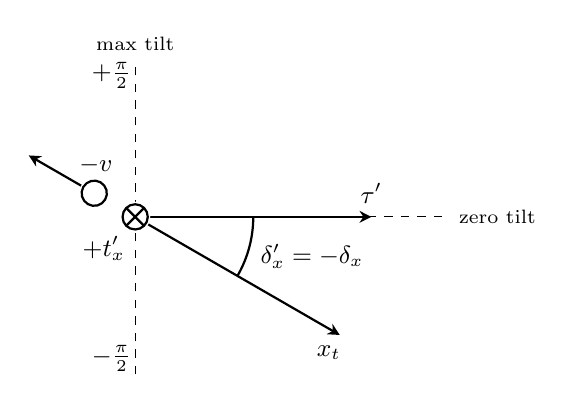
\begin{tikzpicture}[scale=2]
        \tikzset{axis/.style={-{Stealth[length=1.5mm, width=1.5mm]}, thick}}
        % i and j axes
        \draw[dashed] (0,-{2*abs(sin(30))}) -- (0,{2*abs(sin(30))});
        \draw[dashed] (0,0) -- (2,0);
        \node at (2+0.3,0) {\scriptsize zero tilt};
        \node at (0,{0.1+2*abs(sin(30))}) {\scriptsize max tilt};
        \node at (-0.15,{-0.1+2*abs(sin(30))}) {\small $+\frac{\pi}{2}$};   
        \node at (-0.15,{0.1-2*abs(sin(30))}) {\small $-\frac{\pi}{2}$};
        
        \draw[axis] (0,0) -- (1.5,0) node at (1.5,0.15) {\small $\tau'$};
        \draw[axis] (0,0) -- (-30:1.5) node at (-35:1.5) {\small $x_t$};
        \draw[thick] (0.75,0) arc [start angle=0, delta angle=-30, radius=0.75];
        \node at (-25/2:1.15) {\small $\delta_x'=-\delta_x$};
        
        \begin{scope}[scale=0.8]
      \fill[white] (0,0) circle (0.12);
        \draw[thick] (0,0) circle (0.1);
            \draw[thick] (0,0) -- (0.07,0.07);
            \draw[thick] (0,0) -- (-0.07,-0.07);
            \draw[thick] (0,0) -- (0.07,-0.07);
            \draw[thick] (0,0) -- (-0.07,0.07);
            \node at (-0.25,-0.25) {\small $+t_x'$};
        \end{scope}
        
        \begin{scope}[shift={(-30:-0.7)}, rotate=-30, scale=0.8]
        \draw[axis] (0.6,0) -- (-0.1,0);        
        \fill[white] (0.5,0) circle (0.12);
        \draw[thick] (0.5,0) circle (0.1);
            \node at (0.4,0.2) {\small $-v$};
        \end{scope}
        	\end{tikzpicture}
	\caption*{\footnotesize $\mathcal{O}_2, K'$, Spatial Vantage Tilt {\em (looking rightward)}}
\end{minipage}
\end{figure}

\begin{figure}
\begin{minipage}{0.5\textwidth}
	\centering
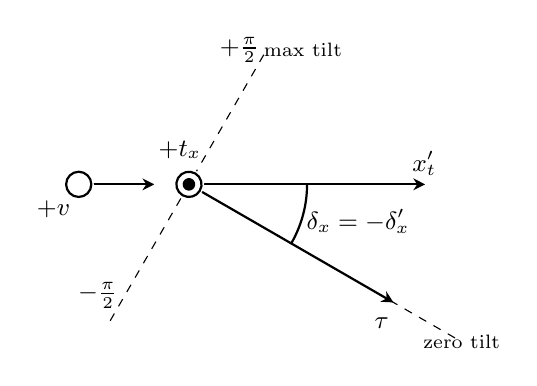
\begin{tikzpicture}[scale=2]
	\begin{scope}[rotate=-30]
        \tikzset{axis/.style={-{Stealth[length=1.5mm, width=1.5mm]}, thick}}
        % i and j axes
        \draw[dashed] (0,-{2*abs(sin(30))}) -- (0,{2*abs(sin(30))});
        \draw[dashed] (0,0) -- (2,0);
        \node at (2,0) {\scriptsize zero tilt};
        \node at (0.2,{0.1+2*abs(sin(30))}) {\scriptsize max tilt};
        \node at (-0.15,{-0.1+2*abs(sin(30))}) {\small $+\frac{\pi}{2}$};   
        \node at (-0.15,{0.1-2*abs(sin(30))}) {\small $-\frac{\pi}{2}$};
        
        \draw[axis] (0,0) -- (1.5,0) node at (1.5,-0.15) {\small $\tau$};
        \draw[axis] (0,0) -- (30:1.5) node at (35:1.5) {\small $x_t'$};
        \draw[thick] (0.75,0) arc [start angle=0, delta angle=30, radius=0.75];
        \node at (35/2:1.1) {\small $\delta_x=-\delta_x'$};
        
        \begin{scope}[scale=0.8]
        \fill[white] (0,0) circle (0.12);
        \draw[thick] (0,0) circle (0.1);
            \fill[black] (0,0) circle (0.05);
            \node at (-0.2,0.2) {\small $+t_x$};
        \end{scope}
        
        \begin{scope}[shift={(30:-0.7)}, rotate=30, scale=0.8]
        \draw[axis] (0,0) -- (0.6,0);        
        \fill[white] (0,0) circle (0.12);
        \draw[thick] (0,0) circle (0.1);
            \node at (-0.2,-0.2) {\small $+v$};
        \end{scope}
        \end{scope}
\end{tikzpicture}
	\caption*{\footnotesize $\mathcal{O}_1, K$, Spatial Vantage Tilt, rotated by $-\delta_x$}
\end{minipage}
\hfill
\begin{minipage}{0.5\textwidth}
	\centering
	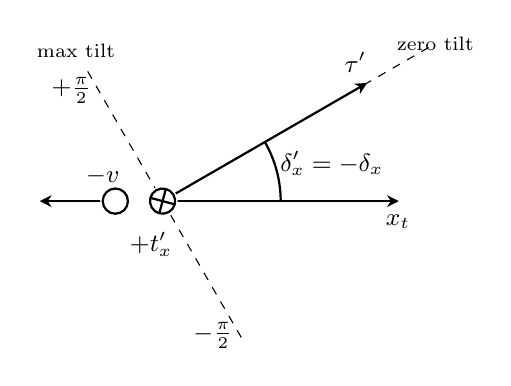
\begin{tikzpicture}[scale=2]
	\begin{scope}[rotate=30]
        \tikzset{axis/.style={-{Stealth[length=1.5mm, width=1.5mm]}, thick}}
        % i and j axes
        \draw[dashed] (0,-{2*abs(sin(30))}) -- (0,{2*abs(sin(30))});
        \draw[dashed] (0,0) -- (2,0);
        \node at (2,0) {\scriptsize zero tilt};
        \node at (0,{0.1+2*abs(sin(30))}) {\scriptsize max tilt};
        \node at (-0.15,{-0.1+2*abs(sin(30))}) {\small $+\frac{\pi}{2}$};   
        \node at (-0.15,{0.1-2*abs(sin(30))}) {\small $-\frac{\pi}{2}$};
        
        \draw[axis] (0,0) -- (1.5,0) node at (1.5,0.15) {\small $\tau'$};
        \draw[axis] (0,0) -- (-30:1.5) node at (-35:1.5) {\small $x_t$};
        \draw[thick] (0.75,0) arc [start angle=0, delta angle=-30, radius=0.75];
        \node at (-35/2:1.1) {\small $\delta_x'=-\delta_x$};
        
        \begin{scope}[scale=0.8]
      \fill[white] (0,0) circle (0.12);
        \draw[thick] (0,0) circle (0.1);
            \draw[thick] (0,0) -- (0.07,0.07);
            \draw[thick] (0,0) -- (-0.07,-0.07);
            \draw[thick] (0,0) -- (0.07,-0.07);
            \draw[thick] (0,0) -- (-0.07,0.07);
            \node at (-0.25,-0.25) {\small $+t_x'$};
        \end{scope}
        
        \begin{scope}[shift={(-30:-0.7)}, rotate=-30, scale=0.8]
        \draw[axis] (0.6,0) -- (-0.1,0);        
        \fill[white] (0.5,0) circle (0.12);
        \draw[thick] (0.5,0) circle (0.1);
            \node at (0.4,0.2) {\small $-v$};
        \end{scope}
        \end{scope}
        	\end{tikzpicture}
	\caption*{\footnotesize $\mathcal{O}_2, K'$, Temporal Vantage Tilt, rotated by $+\delta_x$}
\end{minipage}
\end{figure}

\clearpage
\noindent {\bf Note:}
{\small 
\begin{adjustwidth}{2em}{0pt}
The $(t_y, y_t)$ tilt diagram is structurally identical to the  $(t_x, x_t)$ case, differing only in axis label. For $(t_z, z_t)$, the tilt behaves the same geometrically, but due to the cross product convention used for right-handed $\mathbb{R}^3$ subspaces in $\mathbb{R}^7$, we invert the orientation of the fixed $\tau$ and $z_t$ axes (i.e., $\tau$ and $z_t$ alternate between into/out of the page). This preserves frame consistency across dimensions.\\
\end{adjustwidth}}

\noindent Designating the train's speed as being in the x direction, the $K$ and $K'$ observer frames reduce in the usual case to:
\begin{flalign*}
\quad&\text{\small Observer 1 $(\mathcal{O}_1)$, Minkowski Embankment Frame,} k&&\\[-2mm]
\quad&k=(t, x)&&\\[-2mm]
\quad&\text{\small Observer 1 at relative velocity $-v$ along $x$ with respect to Observer 2}&&\\
\quad&\text{\small Observer 2 $(\mathcal{O}_2)$, Minkowski Train Frame } k'&&\\[-2mm]
\quad&k'=(t', x')&&\\[-2mm]
\quad&\text{\small Observer 2 at relative velocity $+v$ along $x$ with respect to Observer 1}&&
\end{flalign*}
Embankment observer (Observer 1) is stationary in frame $k$. Each observer has a lightclock consisting of two mirrors that they confirmed ahead of time to be of distance length $L$ in their rest frame, perpendicular to agreed motion. Train observer (Observer 2) is moving at velocity $v=\beta c$ relative to embankment, in frame $k'$. Light bounces vertically between mirrors, perpendicular to their direction of motion.\\
\\
\noindent Now the procedure is to apply the occupant vantage tilt by the O-cross-I framework. We promote the scenario  the appropriate 3D submanifold with coordinates $\{(\tau, t_x), -x_t\}$. Universal turn $\tau$ replaces the standard time $t$ dimension. Paired with dimension $i$ is internal time dimension $t_i$, $(i \in x, z, y)$, where $i$ are the spatial coordinates of motion. So in this 7D context (considering now only temporal vantage tilt), we promote the traditional 2D spacetime vector $(t,x)$ into a three dimensional vantage slice $((\tau, t_x),x_t)$, which is itself a projection from higher $\mathbb{R}^7$ Euclidean space. The procedure for promoting is what we call a {\bf 7-lift}, where a lift itself is just a rotation to align each observer's local clock axis $t_x$ with their perceived proper time. After lifting both unprimed and primed coordinates to the 3D temporal vantage subspace, relativistic effects are derived by projecting back down to Minkowski space, via the {\bf 7-squeeze}. Thus, rather than introducing contraction or dilation as distortions, we represent them as the results of standard rotations acting on frames in 7D manifold projected subspaces.\\
\\
\noindent In the O-cross-I framework, time dilation for the light clock train experiment arises from an angular difference between observer vantage coordinates in the $(\tau, t_x)$ plane. The tilt angle $\alpha_x$ introduced above, represents how much an individual observer's local clock vector $t_x$ tilts away from the universal observer clock vector $\tau$.\\
\\
Note, when working in 7D space, we use subscript $t$ on $x, y, z$ like $x_t, y_t, z_t$, and this is to avoid confusion between the usual Minkowki space and the lifted 7D space consisting of $\tau$ and conjugate coordinate pairs $(i_t, t_i)$. We will also adhere to the convention where capital $K$ and $K'$ are the respective lifted frames of $k, k'$ up to the 7D context. Finally, we adhere to a convention where, a rotated frame (say from $K'$ to $K$), will be denoted by a star like $K^*$ and ${K^*}'$. That is, if $k$ is lifted to $K$, and $K$ is rotated such that it matches $K'$, we keep track of which frame variables are relevant by denoting the rotated from $K$ matching $K'$ as $K^*$. The whole point of General Peace Dynamics is to include both observer and individual, thus we take pains to make sure referential vantages are distinguished from one another clearly. For example, Observer 1 in k, considering the Train Frame k' by rotating their point of view from the embankment is emphatically NOT equivalent to Observer 2 considering their train frame in terms of Observer 1. This fact is usually apparent in seemingly benign ad hoc rules of thumb such as, 'reverse sign of velocity to get the inverse of the Lorentz Transform'.\\
 \\
\noindent 
\renewcommand{\arraystretch}{1.5}
\setlength{\arraycolsep}{4pt} 
\subsection*{Mathematical Introduction: 7-Lift, Rotate, 7-Squeeze}
To set the stage for presenting the vantage tilt derivations of Lorentz transform and associated time dilation / length contraction, we now review basic rotation in 3 dimensional Euclidean space. The standard 3 dimensional rotation matrices are for reminder:
\begin{flalign*}
R_x^{(\theta)} &=
\begin{pmatrix}
\begin{array}{r@{}lr@{}lr@{}l}
\phantom{/}&1 & &0 & &0\\
&0 & &\cos\theta & -&\sin\theta \\
&0 & &\sin\theta & &\cos\theta \phantom{/}
\end{array}
\end{pmatrix};\quad
R_y^{(\theta)} =
\begin{pmatrix}
\begin{array}{r@{}lr@{}lr@{}l}
&\cos\theta & &0 & &\sin\theta \\
&0 & &1 & &0\\
-&\sin\theta & &0 & &\cos\theta \phantom{/}
\end{array}
\end{pmatrix};\quad
R_z^{(\theta)} =
\begin{pmatrix}
\begin{array}{r@{}lr@{}lr@{}l}
\,\,\,&\cos\theta & -&\sin\theta & &0\phantom{/}\\
&\sin\theta & &\cos\theta & &0\\
&0 & &0 & &1\\
\end{array}
\end{pmatrix}&&
\end{flalign*}
\noindent But since we are working with 3 dimensional slice subspace projections of $\mathbb{R}^7$, we need to be mindful to make sure both the subspace $\mathbb{R}^3$ cross product structures and the $\mathbb{R}^7$ cross product structure align. Our interest here lies in subspaces in the form of $\{\tau, t_i, i\}$. Each 3 dimensional subspace maintains a preferential ordered pair depending on the quantity of interest (time dilation, length contraction, general Lorentz transform), where for the $x$ dimension of the light clock thought experiment, these quantities correspond to 2 dimensional planes of rotation. These will correspond with the standard rotation matrices. Thus, for coordinate axis triples $\tau, t_i, i \,\, ...\,\, i \in x, y, z$ (also providing $y$ and $z$ for completeness), we have the following 3-spaces:
\begin{flalign*}
\begin{array}{lll}
\{(\tau, t_x), -x_t\},\quad& \{\tau), -t_x, (x_t\} \quad &\{-\tau, (t_x, x_t)\}\\
\{(\tau, t_y), -y_t\},\quad& \{\tau), -t_y, (y_t\},\quad &\{-\tau, (t_y, y_t)\}\\
\{(\tau, t_z), +z_t\},\quad& \{\tau), +t_z, (z_t\},\quad &\{+\tau, (t_z, z_t)\}
\end{array}&&
\end{flalign*}
\noindent Note signs, $(t_z, z_t)$ needing no inversion to preserve higher cross product structure. Also note curved brackets emphasizing the rotation plane for each subspace. To avoid confusion of changing signs in usual 3x1 vectors, we encode the left-handedness of $x$ and $y$ directly into the lift and transform rotator matrices:
\begin{flalign*}
R_{t_x x_t}^{(\varphi_x)} &=
\begin{pmatrix}
\begin{array}{r@{}lr@{}lr@{}l}
&1 & &0 & \phantom{+}&0\\
&0 & &\cos\varphi_x & &\sin\varphi_x \\
&0 & -&\sin\varphi_x & &\cos\varphi_x
\end{array}
\end{pmatrix};\,
R_{\tau x_t}^{(\delta_x)} =
\begin{pmatrix}
\begin{array}{r@{}lr@{}lr@{}l}
&\cos\delta_x & &0 & -&\sin\delta_x \\
\phantom{+}&0 & &1 & &0\\
&\sin\delta_x & &0 & &\cos\delta_x
\end{array}
\end{pmatrix};\,
R_{\tau t_x}^{(\alpha_x)} =
\begin{pmatrix}
\begin{array}{r@{}lr@{}lr@{}l}
&\cos\alpha_x & &\sin\alpha_x & &0\\
-&\sin\alpha_x & &\cos\alpha_x & &0\\
&0 & \phantom{+}&0 & &1\\
\end{array}
\end{pmatrix}&&
\end{flalign*}
\begin{flalign*}
R_{t_y y_t}^{(\varphi_y)} &=
\begin{pmatrix}
\begin{array}{r@{}lr@{}lr@{}l}
&1 & &0 & \phantom{+}&0\\
&0 & &\cos\varphi_y & &\sin\varphi_y \\
&0 & -&\sin\varphi_y & &\cos\varphi_y
\end{array}
\end{pmatrix};\,
R_{\tau y_t}^{(\delta_y)} =
\begin{pmatrix}
\begin{array}{r@{}lr@{}lr@{}l}
&\cos\delta_y & &0 & -&\sin\delta_y \\
\phantom{+}&0 & &1 & &0\\
&\sin\delta_y & &0 & &\cos\delta_y
\end{array}
\end{pmatrix};\,
R_{\tau t_y}^{(\alpha_y)} =
\begin{pmatrix}
\begin{array}{r@{}lr@{}lr@{}l}
&\cos\alpha_y & &\sin\alpha_y & &0\\
-&\sin\alpha_y & &\cos\alpha_y & &0\\
&0 & \phantom{+}&0 & &1\\
\end{array}
\end{pmatrix}&&
\end{flalign*}
\begin{flalign*}
R_{t_z z_t}^{(\varphi_z)} &=
\begin{pmatrix}
\begin{array}{r@{}lr@{}lr@{}l}
&1 & \phantom{+}&0 & &0\\
&0 & &\cos\varphi_z & -&\sin\varphi_z \\
&0 & &\sin\varphi_z & &\cos\varphi_z
\end{array}
\end{pmatrix};\,
R_{\tau z_t}^{(\delta_z)} =
\begin{pmatrix}
\begin{array}{r@{}lr@{}lr@{}l}
&\cos\delta_z & &0 & &\sin\delta_z \\
&0 & &1 & \phantom{+}&0\\
-&\sin\delta_z & &0 & &\cos\delta_z
\end{array}
\end{pmatrix};\,
R_{\tau t_z}^{(\alpha_z)} =
\begin{pmatrix}
\begin{array}{r@{}lr@{}lr@{}l}
&\cos\alpha_z & -&\sin\alpha_z & &0\\
&\sin\alpha_z & &\cos\alpha_z & &0\\
\phantom{+}&0 & &0 & &1\\
\end{array}
\end{pmatrix}&&\\
&\phantom{=}
\begin{array}{r@{}lr@{}lr@{}l}
R_{t_i i_t}^{(\varphi_i)} =R_{t_i i_t}^{(-\varphi_i)\intercal}&  \hspace{2.9cm} R_{\tau i_t}^{(\delta_i)} =R_{\tau i_t}^{(-\delta_i)\intercal}& \hspace{2.9cm} R_{\tau t_i}^{(\alpha_i)} &=R_{\tau t_i}^{(-\alpha_i)\intercal}&
\end{array}&&
\end{flalign*}



\noindent For now, we define $\alpha_i$ as the temporal vantage tilt angle for internal time dimensions $t_i \in t_x, t_y, t_z$, $\delta_i$ as the spatial vantage tilt angle for external space dimensions $i_t \in x_t, y_t, z_t$, and $\varphi_i$ the combined spatial-temporal mixed tilt for $(t_i, i)$ intra sector rotation blocks. For now, (pedagogical purposes), we will refrain from providing an explicit definition for these angles.\\

\noindent Next we take (for case of one dimensional motion in $x$ by some $v$ with respect to time $t$), 7-lifted forms of unprimed ($K$ frame, $\mathcal{O}_1$ observing $K'$ in motion with $\mathcal{O}_2$ and their light clock), and primed coordinate frames ($K'$ $\mathcal{O}_2$ on train, observing $\mathcal{O}_1$ in relative reverse motion with lightclock on embankment).

\subsubsection*{The 7-lift:}
Proposition without proof for now, that the well known effects and idiosyncrasies of special relativity are due to lost information in projection inflicted by default limitations of standard physics' choices of space dimensionality, we find that the first challenge by implementing this O-cross-I framework is to promote the standard 3D and 4D Minkowski space to the full 7D Euclidean form. In most cases we will see that it is in fact possible to reconstruct the fully specified (definite) physical picture from the lower squeezed out standard formulation form. That is, we can reconstruct the original thing (the physical scenario) in a way that is free of indeterminacy, or at least resolved well enough to avoid the scenario where the 'higher dimension physics' does little more than transform one convoluted mess to a different convoluted mess (mess of convolution, a priori, the general conserved quantity easily derived by simply looking around at the state of myriad attempts to unify physics).\\

\noindent To start, let's derive the 7-lifted forms, for the three characteristic tilt angles. Note, when we 7-lift from the 'flattened' Minkowski space, we go from 4D to 7D, disregarding of course irrelevant terms by restricting attention to 3D subspace slices. That is, the approach we take assumes that $\mathbb{R}^7$ is RWOT and has been there as nature's preferred structure this whole time. So, if we 7-lift for example along $x$, so $(t', x') \rightarrow (\tau', t_x', x_t')$, then $x_t'$ is lifted, but it is still by rotational transform definition the same $x'$ from the original flattened Minkowski vantage. Also, please note that $\tau$ at this point in the introduction is deliberately vague. We this dimension the `universal time', the `turn', `proper time', etc. This of course is a deliberate overloading for versatility in a context dependent manner.\\

\subsubsection*{The 7-lift, temporal vantage tilt angle:}

Process: Identify the frame of observer vantage, then identify the frame containing individual vantage of interest. In our context, we will use un-prime coordinates to denote the `initial vantage frame'. Note that we do not reserve primes for moving coordinate frames, for this is an inappropriate preferential bias in the context of relativity's spirit. In the case of Einstein's light clock, unprimed is the embankment that the train moves across. Primed, the train moving, or from primed frame's perspective, the train stationary and pushing the embankment backwards at constant velocity.\\

\noindent Choosing frames, primed and unprimed forces defining coordinate axis sense and valence. In the case of our light clock thought experiment, $x$ and $x'$ are parallel, with the same sense. This means that $k$ sees the positive $+v$ of the passing train, whereas $k'$ sees the embankment traveling with equal but opposite negative velocity $-v$. This is important to keep signs straight, because it determines which direction we rotate upon a 7-lift operation.\\

\subsection*{Liftrime reversal and Lorentz Transform in 1D via temporal vantage tilt angle $\alpha$}

Consider, the propositions that relativistic transformations can be represented as simple rotations in the higher 7-dimensional space, where:\\
\\
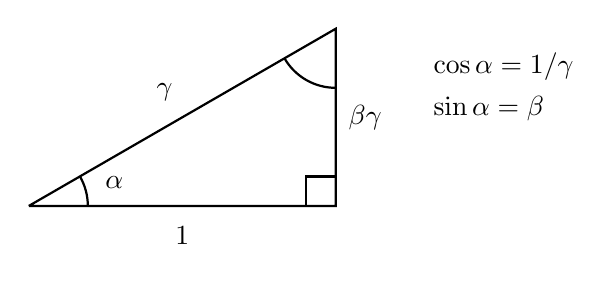
\begin{tikzpicture}[scale=1.5]
    \draw[thick] (0,0)--({3*sqrt(3)/2},0)--({3*sqrt(3)/2},1.5)--(0,0);
    \draw[thick] (0.5,0) arc [start angle=0, delta angle=30, radius=0.5];
    \draw[thick] ({3*sqrt(3)/2},1) arc [start angle=-90, delta angle=-60, radius=0.5];
    \draw[thick] ({3*sqrt(3)/2-0.25},0)--({3*sqrt(3)/2-0.25},0.25)--({3*sqrt(3)/2},0.25);
    \node at ({3*sqrt(3)/4},-0.25) {$1$};
    \node at ({3*sqrt(3)/2+0.25}, 0.75) {$\beta\gamma$};
    \node at (40:1.5) {$\gamma$};
    \node at (15:0.75) {$\alpha$};
    \node at (4,1) {
    $\begin{aligned}
    &\cos\alpha=1/\gamma\\
    &\sin\alpha=\beta
    \end{aligned}$};
\end{tikzpicture}\\[-2mm]

\noindent Where $\beta=v/c$ is the relative velocity as a fraction of light speed, and $\gamma=1/\sqrt{1-\beta^2}$ is the Lorentz factor. We may validate this using the Pythagorean identity:
\begin{flalign*}
\cos^2\alpha + \sin^2\alpha &= 1&&\\
(1/\gamma)^2 + \beta^2 &= 1\\
(1/\gamma)^2 &= 1 - \beta^2\\
\gamma &= \frac{1}{\sqrt{1 - \beta^2}}
\end{flalign*}
\noindent The reason for this choice is that $\alpha$ represents the ``occupant vantage tilt'' between reference frames for individuals (and observers) in our higher-dimensional $\mathbb{R}^7$ space, where:
\begin{itemize}
\item[.]The adjacent side of length $1$ represents the rest frame;
\item[.]The opposite side of length $\beta\gamma$ represents the velocity-dependent distortion;
\item[.]The hypotenuse of length $\gamma$ represents the relativistic distortion factor (here, the temporal).
\end{itemize}
\noindent This geometric representation enables one to replace hyperbolic functions in Minkowski space with simple Euclidean rotations in the extended 7-dimensional space, making relativistic transformations more intuitively accessible, while preserving their standard mathematical structure.\\
\\
\noindent Next, this choice in trigonometric function definition will be demonstrated by applying the 7-lifts to the standard $x$ and $x'$ dimensional light-clock setup, then rotate to and from primed and unprimed frames, and finally to project back down to standard Minkowski spacetime, where the standard Lorentz transformations are recovered:
\begin{flalign*}
&t'=\gamma(t \pm \frac{vx}{c^2})&&\\
&x'=\gamma(x \pm vt)&&
\end{flalign*}


%%%%%%%%%%%%%%%%%




\begin{flalign*}
K_{\{\tau, t_x, x_t\}}^{(t, x)} =
\begin{pmatrix}
\tau\\ t_x\\ x_t
\end{pmatrix}_{\!\!K\!\!} =
R_{\tau x_t}^{(+\delta_x)} k_{\{t, x\}}^{(v)} =
R_{\tau x_t}^{(+\delta_x)}
\begin{pmatrix}
t\\ B\\ x
\end{pmatrix}_{\!\!k\!\!} =
\begin{pmatrix}
\begin{array}{r@{}lr@{}lr@{}l}
&\cos\delta_x & & 0 & -&\sin\delta_x\\
&0 & &1 & &0\\
&\sin\delta_x &&0 & &\cos\delta_x\\
\end{array}
\end{pmatrix}
\begin{pmatrix}
t\\ B\\ x
\end{pmatrix}_{\!\!k\!\!}  =
\begin{pmatrix}
\begin{array}{r@{}l}
&t\cos\delta_x - x\sin\delta_x\\
&B\\
&t\sin\delta_x + x\cos\delta_x\\
\end{array}
\end{pmatrix}_{\!\!K\!\!} &&
\end{flalign*}

\begin{flalign*}
{K^*}_{\{\tau', t_x', x_t'\}}^{(t, x)}
\begin{pmatrix}
\tau'\\ t_x'\\ x_t'
\end{pmatrix}_{\!\!K^*\!\!} &=
R_{\tau t_x}^{(-2\delta_x)} K_{\{\tau, t_x, x\}}^{(t,x)} =
R_{\tau t_x}^{(-2\delta_x)}
\begin{pmatrix}
\tau\\ t_x\\ x_t
\end{pmatrix}_{\!\!K\!\!}&&\\
&= \begin{pmatrix}
\begin{array}{r@{}lr@{}lr@{}l}
&\cos2\delta_x & & 0 & &\sin2\delta_x\\
&0 & &1 & &0\\
-&\sin2\delta_x &&0 & &\cos2\delta_x\\
\end{array}
\end{pmatrix}
\begin{pmatrix}
\tau\\ t_x\\ x_t
\end{pmatrix}_{\!\!K\!\!} =
\begin{pmatrix}
\begin{array}{r@{}l}
&\tau \cos2\delta_x + x_t \sin2\delta_x\\
&t_x\\
&x_t \cos2\delta_x - \tau\sin2\delta_x\\
\end{array}
\end{pmatrix}_{\!\!K^*\!\!}&&\\
&= \begin{pmatrix}
\begin{array}{r@{}l}
&t(\cos2\delta_x\cos\delta_x + \sin2\delta_x\sin\delta_x) - x(\cos2\delta_x\sin\delta_x - \sin2\delta_x\cos\delta_x)\\
&B\\
&x(\cos2\delta_x\cos\delta_x + \sin2\delta_x\sin\delta_x) + t(\cos2\delta_x\sin\delta_x - \sin2\delta_x\cos\delta_x)\\
\end{array}
\end{pmatrix}_{\!\!K^*\!\!}&&\\
&= \begin{pmatrix}
\begin{array}{r@{}l}
&t\cos\delta_x + x\sin\delta_x\\
&B\\
&x\cos\delta_x - t\sin\delta_x\\
\end{array}
\end{pmatrix}_{\!\!K^*\!\!}&&
\end{flalign*}

\begin{flalign*}
{k'}_{\{t', x'\}}^{(v)} =
\begin{pmatrix}
t'\\ x'
\end{pmatrix}_{\!\!k'\!\!} &=
\pi^-(+\delta)
\begin{pmatrix}
\tau'\\ t_x'\\ x_t'
\end{pmatrix}_{\!\!K^*\!\!} =
\begin{pmatrix}
\begin{array}{r@{}lr@{}lr@{}l}
&1 & &\tan\delta_x & \frac{1}{c}&\tan\delta_x\\
&1 & &\tan\delta_x & c&\tan\delta_x\\
\end{array}
\end{pmatrix}
\begin{pmatrix}
\tau'\\ t_x'\\ x_t'
\end{pmatrix}_{\!\!K^*\!\!} =
\begin{pmatrix}
\begin{array}{r@{}lr@{}lr@{}l}
&1 & &\lambda & \frac{1}{c}&\lambda\\
&1 & &\lambda & c&\lambda\\
\end{array}
\end{pmatrix}
\begin{pmatrix}
\begin{array}{r@{}l}
&t\cos\delta_x + x\sin\delta_x\\
&B\\
&x\cos\delta_x - t\sin\delta_x\\
\end{array}
\end{pmatrix}_{\!\!K^*\!\!} &&\\
&= \begin{pmatrix}
\begin{array}{r@{}l}
&t\cos\delta_x + x \sin\delta_x + B\lambda +x \frac{\lambda}{c}\cos\delta_x - t \frac{\lambda}{c}\sin\delta_x\\
&t\cos\delta_x + x \sin\delta_x + B\lambda +x \lambda c \cos\delta_x - t \lambda c \sin\delta_x\\
\end{array}
\end{pmatrix}_{\!\!k'\!\!} &&\\
&= \begin{pmatrix} \begin{array}{r@{}l}
&t\beta_v + x\frac{1}{\gamma_v} + \lambda(x \frac{\beta_v}{c} - t \frac{1}{c\gamma_v}) + B \lambda\\
&t\beta_v + x\frac{1}{\gamma_v} + \lambda(x c\beta_v - t\frac{c}{\gamma_v}) + B \lambda\\
\end{array} \end{pmatrix}_{\!\!k'\!\!}  \quad\quad \cos\delta_x=\beta_v \,\,;\,\, \sin\delta_x=\frac{1}{\gamma_v} \quad\quad&&\\
&= \begin{pmatrix} \begin{array}{r@{}l}
&t(\beta_v - \frac{1}{c\beta_v\gamma_v^2})+ x(\frac{1}{\gamma_v} + \frac{1}{c\gamma_v}) + B \frac{1}{\beta_v\gamma_v}\\
&t(\beta_v  - \frac{c}{\beta_v\gamma_v^2}) + x(\frac{1}{\gamma_v} + \frac{c}{\gamma_v}) + B\frac{1}{\beta_v\gamma_v}\\
\end{array} \end{pmatrix}_{\!\!k'\!\!}  \quad\quad \lambda=\frac{1}{\beta_v\gamma_v}&&\\
&= \begin{pmatrix} \begin{array}{r@{}l}
&t(\beta_v - \frac{1}{c\beta_v\gamma_v^2})+ x(\frac{1}{\gamma_v} + \frac{1}{c\gamma_v}) + B \frac{1}{\beta_v\gamma_v}\\
&t(\beta_v  - \frac{c}{\beta_v\gamma_v^2}) + x(\frac{1}{\gamma_v} + \frac{c}{\gamma_v}) + B\frac{1}{\beta_v\gamma_v}\\
\end{array} \end{pmatrix}_{\!\!k'\!\!}  \quad\quad \lambda=\frac{1}{\beta_v\gamma_v}&&\\
&= \begin{pmatrix} \begin{array}{r@{}l}
&t(\beta_v - \frac{\beta_v}{c})+ x(\frac{1}{\gamma_v} + \lambda\frac{\beta_v}{c}) + B \lambda\\
&t(\beta_v  - \lambda\frac{c}{\gamma_v}) + x(\frac{1}{\gamma_v} + \lambda c\beta_v) + B \lambda\\
\end{array} \end{pmatrix}_{\!\!k'\!\!}  \quad\quad \lambda=\beta_v\gamma_v&&\\
&= \begin{pmatrix}
\begin{array}{r@{}l}
&\frac{1}{\gamma}\left(t(\frac{c\beta^2\gamma^2 - 1}{c\beta\gamma}) + x(\frac{c+1}{c}) + B \frac{1}{\beta}\right)\\
&\frac{1}{\gamma}\left(t(\frac{\beta^2\gamma^2 - c}{\beta\gamma}) + x(c+1) + B \frac{1}{\beta}\right)\\
\end{array}
\end{pmatrix}_{\!\!k'\!\!}&&\\
&+++++++++++++++++++++++++++++++++&&\\
\end{flalign*}

\begin{flalign*}
\frac{d}{dv}
\begin{pmatrix}
t'\\ x'
\end{pmatrix} &=
\frac{d}{dv}
\begin{pmatrix}
\begin{array}{r@{}l}
& \gamma_v(t - \frac{vx}{c^2})\\
& \gamma_v(x - vt)\\
\end{array}
\end{pmatrix} \quad\quad \frac{d}{dv}\gamma_v = \frac{v\gamma_v^3}{c^2}&&\\
&= \begin{pmatrix} \begin{array}{r@{}l}
& \frac{d\gamma_v}{dv}(t - x \frac{v}{c^2}) - x \frac{\gamma_v}{c^2}\\
& \frac{d\gamma_v}{dv}(x - vt) - t \gamma_v\\
\end{array} \end{pmatrix}&&\\
&= \begin{pmatrix} \begin{array}{r@{}l}
& t \frac{v\gamma_v^3}{c^2} - x \frac{\gamma_v}{c^2}(\beta_v^2\gamma_v^2 + 1)\\
& x \frac{v\gamma_v^3}{c^2} - t \gamma_v(\beta_v^2\gamma_v^2 + 1)\\
\end{array} \end{pmatrix} \quad\quad \Leftarrow  \beta_v^2\gamma_v^2 + 1 = \gamma_v^2&&\\
&= \begin{pmatrix} \begin{array}{r@{}l}
& t  \frac{v}{c^2}\gamma_v^3  - x \frac{\gamma_v^3}{c^2}\\
& x \frac{v}{c^2}\gamma_v^3 - t\gamma_v^3\\
\end{array} \end{pmatrix}
=  \begin{pmatrix} \begin{array}{r@{}l}
&\frac{\gamma_v^3}{c} \left(\beta_v t  - \frac{1}{c} x \right)\\
& \frac{\gamma_v^3}{c}\left(\beta_v x - ct\right)\\
\end{array} \end{pmatrix}
=  \begin{pmatrix} \begin{array}{r@{}l}
&\frac{\gamma_v^3}{c^2} \left(v t  - x \right)\\
& \frac{\gamma_v^3}{c^2}\left(v x - c^2t \right)\\
\end{array} \end{pmatrix}
=  \begin{pmatrix} \begin{array}{r@{}l}
&\frac{1}{v}\frac{d\gamma_v}{dv} \left(v t  - x \right)\\
&\frac{1}{v}\frac{d\gamma_v}{dv}\left(v x - c^2 t \right)\\
\end{array} \end{pmatrix}
=  \begin{pmatrix} \begin{array}{r@{}l}
&(\partial_v\gamma_v) \left(t  - \frac{x}{v} \right)\\
&(\partial_v\gamma_v) \left(x - c^2 \frac{t}{v} \right)\\
\end{array} \end{pmatrix}&&\\
\begin{pmatrix}
\frac{dt'}{d\gamma_v}\\ \frac{dx'}{d\gamma_v}
\end{pmatrix} 
&=  \begin{pmatrix} \begin{array}{r@{}l}
&t  - \frac{x}{v}\\
&x -  \frac{c^2t}{v}\\
\end{array} \end{pmatrix}&&\\
\begin{pmatrix}
\frac{dt'}{d\delta_x}\\ \frac{dx'}{d\delta_x}
\end{pmatrix} 
&=  \begin{pmatrix} \begin{array}{r@{}l}
&t  - \frac{\alpha_x x}{c}\\
&x -  c\alpha_x t\\
\end{array} \end{pmatrix}&&\\
\end{flalign*}

\begin{flalign*}
&= \begin{pmatrix} \begin{array}{r@{}l}
&t\cos\delta_x + x \sin\delta_x + B\lambda +x\lambda\frac{1}{c}\cos\delta_x - t \lambda\frac{1}{c}\sin\delta_x\\
&t\cos\delta_x + x \sin\delta_x + B\lambda +x\lambda c \cos\delta_x - t \lambda c \sin\delta_x\\
\end{array} \end{pmatrix}_{\!\!k'\!\!} &&\\
&= \begin{pmatrix} \begin{array}{r@{}l}
&t\beta_v + x\frac{1}{\gamma_v} + \lambda(x \frac{\beta_v}{c} - t \frac{1}{c\gamma_v}) + B \lambda\\
&t\beta_v + x\frac{1}{\gamma_v} + \lambda(x c\beta_c - t\frac{c}{\gamma_c}) + B \lambda\\
\end{array} \end{pmatrix}_{\!\!k'\!\!} \quad\quad \cos\delta_x=\beta_v \,\,;\,\, \sin\delta_x=\frac{1}{\gamma_v} \quad\quad&&\\
&= \begin{pmatrix} \begin{array}{r@{}l}
&t(\beta_v - \frac{1}{c\beta_v\gamma_v^2}) + x (\frac{1}{\gamma_v} - \frac{1}{c\gamma_v}) + B \frac{1}{\beta_v\gamma_v}\\
&t(\beta_v - \frac{c}{\beta_v\gamma_v^2}) + x (\frac{1}{\gamma_v} - \frac{c}{\gamma_v}) + B \frac{1}{\beta_v\gamma_v}\\
\end{array} \end{pmatrix}_{\!\!k'\!\!} \quad\quad \lambda=\frac{1}{\beta_v\gamma_v}&&\\
&= \begin{pmatrix} \begin{array}{r@{}l}
&\frac{1}{\gamma_v}(t(\frac{c\beta_v^2\gamma_v^2 - 1}{c\beta_v\gamma_v}) + x (\frac{c+1}{c})+ B \frac{1}{\beta_v}\\
&\frac{1}{\gamma_v}(t(\frac{\beta_v^2\gamma_v^2 - c}{\beta_v\gamma_v}) + x (c+1) + B \frac{1}{\beta_v}\\
\end{array} \end{pmatrix}_{\!\!k'\!\!} &&\\
\end{flalign*}
fgbegrbnrgnfgn
\begin{flalign*}
&= \begin{pmatrix} \begin{array}{r@{}l}
&t\beta_v + x\frac{1}{\gamma_v} + \lambda(x \frac{\beta_v}{c} - t \frac{1}{c\gamma_v}) + B \lambda\\
&t\beta_v + x\frac{1}{\gamma_v} + \lambda(x c\beta_c - t\frac{c}{\gamma_c}) + B \lambda\\
\end{array} \end{pmatrix}_{\!\!k'\!\!} \quad\quad \cos\delta_x=\beta_v \,\,;\,\, \sin\delta_x=\frac{1}{\gamma_v} \quad\quad&&\\
&= \begin{pmatrix} \begin{array}{r@{}l}
&t\beta_v + x\frac{1}{\gamma_v} + x \frac{\gamma_v}{c} - t \frac{\beta_v}{c}) - B \frac{\beta_v}{\gamma_v}\\
&t\beta_v + x\frac{1}{\gamma_v} + \lambda(x c\beta_c - t\frac{c}{\gamma_c}) - B \frac{\beta_v}{\gamma_v}\\
\end{array} \end{pmatrix}_{\!\!k'\!\!} \lambda=\frac{\gamma_v}{\beta_v}=-\frac{\gamma^2}{v}&&\\
&= \begin{pmatrix} \begin{array}{r@{}l}
&t(\beta_v - \frac{1}{c\beta_v\gamma_v^2}) + x (\frac{1}{\gamma_v} - \frac{1}{c\gamma_v}) + B \frac{1}{\beta_v\gamma_v}\\
&t(\beta_v - \frac{c}{\beta_v\gamma_v^2}) + x (\frac{1}{\gamma_v} - \frac{c}{\gamma_v}) + B \frac{1}{\beta_v\gamma_v}\\
\end{array} \end{pmatrix}_{\!\!k'\!\!} \quad\quad \lambda=\frac{\gamma_v}{\beta_v}=-\frac{\gamma^2}{v}&&\\
&= \begin{pmatrix} \begin{array}{r@{}l}
&t(\beta_v - \frac{1}{c\beta_v\gamma_v^2}) + x (\frac{1}{\gamma_v} - \frac{1}{c\gamma_v}) + B \frac{1}{\beta_v\gamma_v}\\
&t(\beta_v - \frac{c}{\beta_v\gamma_v^2}) + x (\frac{1}{\gamma_v} - \frac{c}{\gamma_v}) + B \frac{1}{\beta_v\gamma_v}\\
\end{array} \end{pmatrix}_{\!\!k'\!\!} 
&= \begin{pmatrix} \begin{array}{r@{}l}
&\frac{1}{\gamma_v}(t(\frac{c\beta_v^2\gamma_v^2 - 1}{c\beta_v\gamma_v}) + x (\frac{c+1}{c})+ B \frac{1}{\beta_v}\\
&\frac{1}{\gamma_v}(t(\frac{\beta_v^2\gamma_v^2 - c}{\beta_v\gamma_v}) + x (c+1) + B \frac{1}{\beta_v}\\
\end{array} \end{pmatrix}_{\!\!k'\!\!} &&\\
\end{flalign*}




%%%%%%%%%%%%%%%%


\noindent (Where the sign depends on the direction of the relative motion between reference frames, chosen by the physicist, per standard transform conventions.) This is the introduction that illustrates the thesis of General Peace Dynamics: non-linear and paradoxical elements of the usual special and genera relativity, plus those residing in the field of quantum physics, plus others, may be understood geometrically as rotations in the higher 7-dimensional Euclidean space by a positive definite metric, rather than requiring hyperbolic transformations, else.\\
\\
\noindent First, 7-lift $k$ and $k'$ to 7D space, frames $K$ and $K'$, respectively:\\
\begin{flalign*}
K_{\{\tau, t_x, x_t\}}^{(t, x)} =
\begin{pmatrix}
\tau\\ t_x\\ x_t
\end{pmatrix}_{\!\!K\!\!} =
R_{\tau t_x}^{(+\alpha_x)} k_{\{t, x\}}^{(v)} =
R_{\tau t_x}^{(+\alpha_x)}
\begin{pmatrix}
t\\ A\\ x
\end{pmatrix}_{\!\!k\!\!}  =
\begin{pmatrix}
\begin{array}{r@{}lr@{}lr@{}l}
&\cos\alpha_x & &\sin\alpha_x & &0\\
-&\sin\alpha_x & &\cos\alpha_x & &0\\
&0 & \phantom{+}&0 & &1\\
\end{array}
\end{pmatrix}
\begin{pmatrix}
t\\ A\\ x
\end{pmatrix}_{\!\!k\!\!}  =
\begin{pmatrix}
\begin{array}{r@{}l}
&t\cos\alpha_x + A\sin\alpha_x\\
&A\cos\alpha_x - t\sin\alpha_x\\
&x\\
\end{array}
\end{pmatrix}_{\!\!K\!\!} &&
\end{flalign*}

\begin{flalign*}
{K'}_{\{\tau', t_x', x_t'\}}^{(t', x')} =
\begin{pmatrix}
\tau'\\ t_x'\\ x_t'
\end{pmatrix}_{\!\!K'\!\!} =
R_{\tau t_x}^{(-\alpha_x)} {k'}_{\{t', x'\}}^{(v')} =
R_{\tau t_x}^{(-\alpha_x)}
\begin{pmatrix}
t'\\ A'\\ x'
\end{pmatrix}_{\!\!k'\!\!} =
\begin{pmatrix}
\begin{array}{r@{}lr@{}lr@{}l}
&\cos\alpha_x & -&\sin\alpha_x & &0\\
&\sin\alpha_x & &\cos\alpha_x & &0\\
&0 & \phantom{+}&0 & &1\\
\end{array}
\end{pmatrix}
\begin{pmatrix}
t'\\ A'\\ x'
\end{pmatrix}_{\!\!k'\!\!} =
\begin{pmatrix}
\begin{array}{r@{}l}
&t'\cos\alpha_x - A'\sin\alpha_x\\
&A'\cos\alpha_x + t'\sin\alpha_x\\
&x'\\
\end{array}
\end{pmatrix}_{\!\!K'\!\!}&&
\end{flalign*}
\\
\noindent Note, we inject a parameter $A$ and $A'$ to demonstrate that we can use the standard 3D rotation matrices with no consequence, while also reserving space in the 7-lift for additional physical quantity to lift in tandem, should that become relevant. The alternative is to use a simple inverse projection matrix. For now, one could think of $A$ and $A'$ as a phase term that cancels out in a wash after 7-squeeze completes.\\
\\
\noindent Next, we take each lifted frame, and rotate it by double angle $\alpha$. This takes the frame's velocity, rotates by one $\alpha$ to reach zero mutual velocity (or the middle observer frame) then pass by another $\alpha$ to reach the opposite prime frame's velocity: 

\begin{flalign*}
{K^*}_{\{\tau', t_x', x_t'\}}^{(t, x)}
\begin{pmatrix}
\tau'\\ t_x'\\ x_t'
\end{pmatrix}_{\!\!K^*\!\!} &=
R_{\tau t_x}^{(-2\alpha_x)} K_{\{\tau, t_x, x\}}^{(t,x)} =
R_{\tau t_x}^{(-2\alpha_x)}
\begin{pmatrix}
\tau\\ t_x\\ x_t
\end{pmatrix}_{\!\!K\!\!}&&\\
&= \begin{pmatrix}
\begin{array}{r@{}lr@{}lr@{}l}
&\cos2\alpha_x & -&\sin2\alpha_x & &0\\
+&\sin2\alpha_x & &\cos2\alpha_x & &0\\
&0 & \phantom{+}&0 & &1\\
\end{array}
\end{pmatrix}
\begin{pmatrix}
\tau\\ t_x\\ x_t
\end{pmatrix}_{\!\!K\!\!} =
\begin{pmatrix}
\begin{array}{r@{}l}
&\tau\cos2\alpha_x - t_x\sin2\alpha_x\\
&t_x\cos2\alpha_x + \tau\sin2\alpha_x\\
&x_t\\
\end{array}
\end{pmatrix}_{\!\!K^*\!\!}&&\\
&= \begin{pmatrix}
\begin{array}{r@{}l}
&t(\cos2\alpha_x\cos\alpha_x + \sin2\alpha_x\sin\alpha_x) + A(\cos2\alpha_x\sin\alpha_x - \sin2\alpha_x\cos\alpha_x)\\
&A(\cos2\alpha_x\cos\alpha_x + \sin2\alpha_x\sin\alpha_x) - t(\cos2\alpha_x\sin\alpha_x - \sin2\alpha_x\cos\alpha_x)\\
&x\\
\end{array}
\end{pmatrix}_{\!\!K^*\!\!}&&\\
&= \begin{pmatrix}
\begin{array}{r@{}l}
&t\cos\alpha_x - A\sin\alpha_x\\
&A\cos\alpha_x + t\sin\alpha_x\\
&x\\
\end{array}
\end{pmatrix}_{\!\!K^*\!\!}&&
\end{flalign*}

\begin{flalign*}
{{K'}^*}_{\{\tau, t_x, x_t\}}^{(t', x')}
\begin{pmatrix}
\tau\\ t_x\\ x_t
\end{pmatrix}_{\!\!{K'}^*\!\!} &=
R_{\tau t_x}^{(+2\alpha_x)} {K'}_{\{\tau', t_x', x'\}}^{(t',x')} =
R_{\tau t_x}^{(-2\alpha_x)}
\begin{pmatrix}
\tau'\\ t_x'\\ x_t'
\end{pmatrix}_{\!\!{K'}\!\!} &&\\
&= \begin{pmatrix}
\begin{array}{r@{}lr@{}lr@{}l}
&\cos2\alpha_x & +&\sin2\alpha_x & &0\\
-&\sin2\alpha_x & &\cos2\alpha_x & &0\\
&0 & \phantom{+}&0 & &1\\
\end{array}
\end{pmatrix}
\begin{pmatrix}
\tau'\\ t_x'\\ x_t'
\end{pmatrix}_{\!\!K'\!\!}=
\begin{pmatrix}
\begin{array}{r@{}l}
&\tau'\cos2\alpha_x + t_x'\sin2\alpha_x\\
&t_x'\cos2\alpha_x - \tau'\sin2\alpha_x\\
&x_t'\\
\end{array}
\end{pmatrix}_{\!\!{K'}^*\!\!}&&\\
&= \begin{pmatrix}
\begin{array}{r@{}l}
&t'(\cos2\alpha_x\cos\alpha_x + \sin2\alpha_x\sin\alpha_x) - A'(\cos2\alpha_x\sin\alpha_x - \sin2\alpha_x\cos\alpha_x)\\
&A'(\cos2\alpha_x\cos\alpha_x + \sin2\alpha_x\sin\alpha_x) + t'(\cos2\alpha_x\sin\alpha_x - \sin2\alpha_x\cos\alpha_x)\\
&x'\\
\end{array}
\end{pmatrix}_{\!\!{K'}^*\!\!}&&\\
&= \begin{pmatrix}
\begin{array}{r@{}l}
&t'\cos\alpha_x +A'\sin\alpha_x\\
&A'\cos\alpha_x - t'\sin\alpha_x\\
&x'\\
\end{array}
\end{pmatrix}_{\!\!{K'}^*\!\!}&&
\end{flalign*}
\\
\noindent Finally we 7-squeeze each star $K, K'$ rotated frames to see if they produce the usual Lorentz Transform. These represent a final rotation by $\pm\alpha$ corresponding to projection coefficient $\lambda=\pm\beta\gamma$ or, simply $\tan\alpha$.
\begin{flalign*}
{k'}_{\{t', x'\}}^{(v)} =
\begin{pmatrix}
t'\\ x'
\end{pmatrix}_{\!\!k'\!\!} &=
\pi^-(+\alpha)
\begin{pmatrix}
\tau'\\ t_x'\\ x_t'
\end{pmatrix}_{\!\!K^*\!\!} =
\begin{pmatrix}
\begin{array}{r@{}lr@{}lr@{}l}
&1 & &\tan\alpha_x & \frac{1}{c}&\tan\alpha_x\\
&1 & &\tan\alpha_x & c&\tan\alpha_x\\
\end{array}
\end{pmatrix}
\begin{pmatrix}
\tau'\\ t_x'\\ x_t'
\end{pmatrix}_{\!\!K^*\!\!} =
\begin{pmatrix}
\begin{array}{r@{}lr@{}lr@{}l}
&1 & &\lambda & \frac{1}{c}&\lambda\\
&1 & &\lambda & c&\lambda\\
\end{array}
\end{pmatrix}
\begin{pmatrix}
\begin{array}{r@{}l}
&t\cos\alpha_x - A\sin\alpha_x\\
&A\cos\alpha_x + t\sin\alpha_x\\
&x\\
\end{array}
\end{pmatrix}_{\!\!K^*\!\!} &&\\
&= \begin{pmatrix}
\begin{array}{r@{}l}
&t\cos\alpha_x - A\sin\alpha_x + A\lambda\cos\alpha_x +t\lambda\sin\alpha_x + \frac{1}{c}\lambda x\\
&t\cos\alpha_x - A\sin\alpha_x + A\lambda\cos\alpha_x +t\lambda\sin\alpha_x + c\lambda x\\
\end{array}
\end{pmatrix}_{\!\!k'\!\!} &&\\
&= \begin{pmatrix}
\begin{array}{r@{}l}
&t\frac{1}{\gamma} - A\beta + A\frac{\lambda}{\gamma} + t\lambda\beta + \frac{1}{c}\lambda x\\
&t\frac{1}{\gamma} - A\beta + A\frac{\lambda}{\gamma} + t\lambda\beta + c\lambda x\\
\end{array}
\end{pmatrix}_{\!\!k'\!\!} \quad\quad \cos\alpha_x=\frac{1}{\gamma} \,\,;\,\, \sin\alpha_x=\beta\quad\quad&&\\
&= \begin{pmatrix}
\begin{array}{r@{}l}
&\gamma(t + \frac{vx}{c^2})\\
&\gamma(t + vx)\\
\end{array}
\end{pmatrix}_{\!\!k'(v)\!\!} \quad\quad \lambda=\beta\gamma=-\beta'\gamma'&&\\
&= \begin{pmatrix}
\begin{array}{r@{}l}
&\gamma(t - \frac{vx}{c^2})\\
&\gamma(t - vx)\\
\end{array}
\end{pmatrix}_{\!\!k'(v')\!\!}&&
\end{flalign*}

\begin{flalign*}
{k}_{\{t, x\}}^{(v)} =
\begin{pmatrix}
t\\ x
\end{pmatrix}_{\!\!k\!\!} &=
\pi^-(-\alpha)
\begin{pmatrix}
\tau\\ t_x\\ x_t
\end{pmatrix}_{\!\!{K'}^*\!\!} =
\begin{pmatrix}
\begin{array}{r@{}lr@{}lr@{}l}
&1 & &-\tan\alpha_x & -\frac{1}{c}&\tan\alpha_x\\
&1 & &-\tan\alpha_x & -c&\tan\alpha_x\\
\end{array}
\end{pmatrix}
\begin{pmatrix}
\tau\\ t_x\\ x_t
\end{pmatrix}_{\!\!{K'}^*\!\!} =
\begin{pmatrix}
\begin{array}{r@{}lr@{}lr@{}l}
&1 & &\lambda & \frac{1}{c}&\lambda\\
&1 & &\lambda & c&\lambda\\
\end{array}
\end{pmatrix}
\begin{pmatrix}
\begin{array}{r@{}l}
&t'\cos\alpha_x + A'\sin\alpha_x\\
&A'\cos\alpha_x - t'\sin\alpha_x\\
&x'\\
\end{array}
\end{pmatrix}_{\!\!{K'}^*\!\!} &&\\
&= \begin{pmatrix}
\begin{array}{r@{}l}
&t'\cos\alpha_x + A'\sin\alpha_x + A'\lambda\cos\alpha_x - t\lambda\sin\alpha_x + \frac{1}{c}\lambda x\\
&t'\cos\alpha_x + A'\sin\alpha_x + A'\lambda\cos\alpha_x - t\lambda\sin\alpha_x + c\lambda x\\
\end{array}
\end{pmatrix}_{\!\!k\!\!} &&\\
&= \begin{pmatrix}
\begin{array}{r@{}l}
&t\frac{1}{\gamma} + A\beta + A\frac{\lambda}{\gamma} - t\lambda\beta + \frac{1}{c}\lambda x\\
&t\frac{1}{\gamma} + A\beta + A\frac{\lambda}{\gamma} - t\lambda\beta + c\lambda x\\
\end{array}
\end{pmatrix}_{\!\!k\!\!} \quad\quad \cos\alpha_x=\frac{1}{\gamma} \,\,;\,\, \sin\alpha_x=\beta\quad\quad&&\\
&= \begin{pmatrix}
\begin{array}{r@{}l}
&\gamma(t - \frac{vx}{c^2})\\
&\gamma(t - vx)\\
\end{array}
\end{pmatrix}_{\!\!k(v)\!\!} \quad\quad \lambda=-\beta\gamma=\beta'\gamma'&&\\
&= \begin{pmatrix}
\begin{array}{r@{}l}
&\gamma(t + \frac{vx}{c^2})\\
&\gamma(t + vx)\\
\end{array}
\end{pmatrix}_{\!\!k(v')\!\!}&&
\end{flalign*}

\noindent Now, note that the artificially injected $t_x$ component $A$ has no effect on the overall result when we squeeze back down in this manner. We still have yet to determine the significance of $A$.\\
\\
\noindent Referring back to the right triangle used to define $\cos\alpha$ and $\sin\alpha$, we note that we can safely preserve the relationship by dividing through by $\gamma$, thus looking at the picture in terms of hypotenuse $1$, then multiply through by $c$:\\
\\
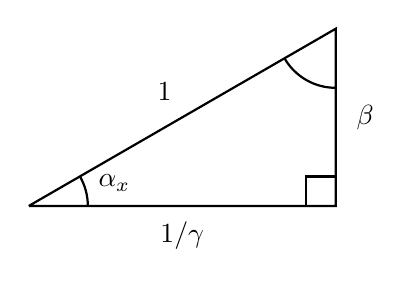
\begin{tikzpicture}[scale=1.5]
    \draw[thick] (0,0)--({3*sqrt(3)/2},0)--({3*sqrt(3)/2},1.5)--(0,0);
    \draw[thick] (0.5,0) arc [start angle=0, delta angle=30, radius=0.5];
    \draw[thick] ({3*sqrt(3)/2},1) arc [start angle=-90, delta angle=-60, radius=0.5];
    \draw[thick] ({3*sqrt(3)/2-0.25},0)--({3*sqrt(3)/2-0.25},0.25)--({3*sqrt(3)/2},0.25);
    \node at ({3*sqrt(3)/4},-0.25) {$1/\gamma$};
    \node at ({3*sqrt(3)/2+0.25}, 0.75) {$\beta$};
    \node at (40:1.5) {$1$};
    \node at (15:0.75) {$\alpha_x$};
\end{tikzpicture}
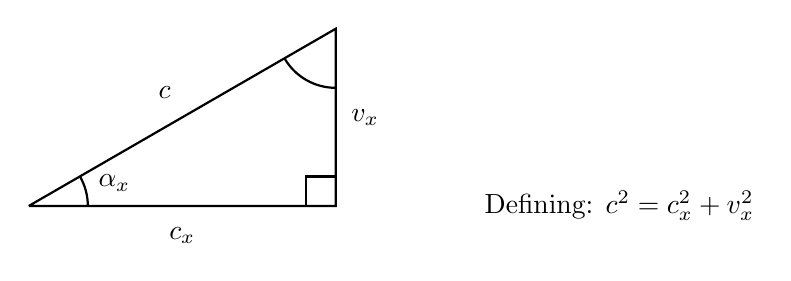
\begin{tikzpicture}[scale=1.5]
    \draw[thick] (0,0)--({3*sqrt(3)/2},0)--({3*sqrt(3)/2},1.5)--(0,0);
    \draw[thick] (0.5,0) arc [start angle=0, delta angle=30, radius=0.5];
    \draw[thick] ({3*sqrt(3)/2},1) arc [start angle=-90, delta angle=-60, radius=0.5];
    \draw[thick] ({3*sqrt(3)/2-0.25},0)--({3*sqrt(3)/2-0.25},0.25)--({3*sqrt(3)/2},0.25);
    \node at ({3*sqrt(3)/4},-0.25) {$c_x$};
    \node at ({3*sqrt(3)/2+0.25}, 0.75) {$v_x$};
    \node at (40:1.5) {$c$};
    \node at (15:0.75) {$\alpha_x$};
    \node at (5,0) {Defining: $c^2=c_x^2+v_x^2$};
\end{tikzpicture}

\noindent As in second triangle, if we we restrict consideration to velocity in the $x$ direction, we can define $\sqrt{c^2-v_x^2}$ as the difference in velocity $c_x$, and we can express each side in terms of the expanded Pythagorean form by:\\
\\
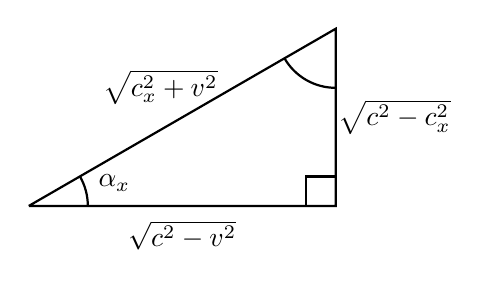
\begin{tikzpicture}[scale=1.5]
    \draw[thick] (0,0)--({3*sqrt(3)/2},0)--({3*sqrt(3)/2},1.5)--(0,0);
    \draw[thick] (0.5,0) arc [start angle=0, delta angle=30, radius=0.5];
    \draw[thick] ({3*sqrt(3)/2},1) arc [start angle=-90, delta angle=-60, radius=0.5];
    \draw[thick] ({3*sqrt(3)/2-0.25},0)--({3*sqrt(3)/2-0.25},0.25)--({3*sqrt(3)/2},0.25);
    \node at ({3*sqrt(3)/4},-0.25) {$\sqrt{c^2-v^2}$};
    \node at ({3*sqrt(3)/2+0.5}, 0.75) {$\sqrt{c^2-c_x^2}$};
    \node at (42:1.5) {$\sqrt{c_x^2+v^2}$};
    \node at (15:0.75) {$\alpha_x$};
\end{tikzpicture}
\begin{flalign*}
\tan\alpha_x = &\frac{\sqrt{c^2-c_x^2}}{\sqrt{c^2-v_x^2}}
=\frac{\sqrt{1-\frac{c_x^2}{c^2}}}{\sqrt{1-\frac{v_x^2}{c^2}}}
=\frac{\gamma_v}{\gamma_c}\quad&
&\text{where}\quad \gamma_v=\frac{1}{\sqrt{1-\frac{v_x^2}{c^2}}}& &\text{and}\quad
\gamma_v=\frac{1}{\sqrt{1-\frac{c_x^2}{c^2}}}&&\\
\text{also}\quad&\sqrt{c_x^2+v_x^2}=\frac{1}{\beta_v \beta_c} \quad& &\text{where}\quad \beta_v=\frac{v_x}{c} & &\text{and} \quad \beta_c=\frac{c_x}{c}&&
\end{flalign*}
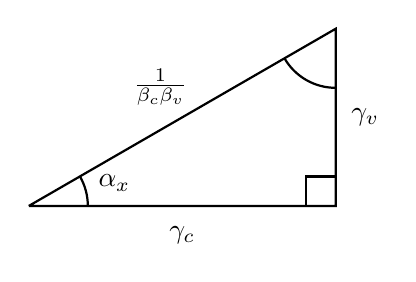
\begin{tikzpicture}[scale=1.5]
    \draw[thick] (0,0)--({3*sqrt(3)/2},0)--({3*sqrt(3)/2},1.5)--(0,0);
    \draw[thick] (0.5,0) arc [start angle=0, delta angle=30, radius=0.5];
    \draw[thick] ({3*sqrt(3)/2},1) arc [start angle=-90, delta angle=-60, radius=0.5];
    \draw[thick] ({3*sqrt(3)/2-0.25},0)--({3*sqrt(3)/2-0.25},0.25)--({3*sqrt(3)/2},0.25);
    \node at ({3*sqrt(3)/4},-0.25) {$\gamma_c$};
    \node at ({3*sqrt(3)/2+0.25}, 0.75) {$\gamma_v$};
    \node at (42:1.5) {$\frac{1}{\beta_c\beta_v}$};
    \node at (15:0.75) {$\alpha_x$};
\end{tikzpicture}\\
\noindent If we follow along with the emerging symmetry, we find ourselves tempted to define the opposite angle as our spatial vantage tilt $\delta_x$, a combined tilt angle as completing right, $\varphi_x$, and inverses of each beta term being $\alpha_x$ and $\delta_x$, so resulting triangle looks like:\\
\\
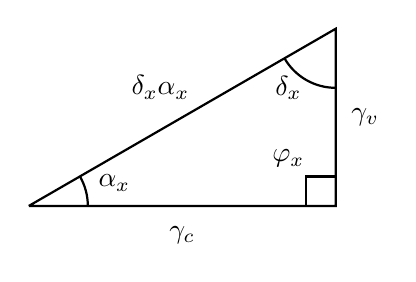
\begin{tikzpicture}[scale=1.5]
    \draw[thick] (0,0)--({3*sqrt(3)/2},0)--({3*sqrt(3)/2},1.5)--(0,0);
    \draw[thick] (0.5,0) arc [start angle=0, delta angle=30, radius=0.5];
    \draw[thick] ({3*sqrt(3)/2},1) arc [start angle=-90, delta angle=-60, radius=0.5];
    \draw[thick] ({3*sqrt(3)/2-0.25},0)--({3*sqrt(3)/2-0.25},0.25)--({3*sqrt(3)/2},0.25);
    \node at ({3*sqrt(3)/4},-0.25) {$\gamma_c$};
    \node at ({3*sqrt(3)/2+0.25}, 0.75) {$\gamma_v$};
    \node at (42:1.5) {$\delta_x\alpha_x$};
    \node at (15:0.75) {$\alpha_x$};
    \node at ({3*sqrt(3)/2-0.4},0.4) {$\varphi_x$};
    \node at ({3*sqrt(3)/2-0.4},1) {$\delta_x$};
\end{tikzpicture}\\
\noindent In terms of our general axis vantage tilt angles, the law of sines produces the resulting relationship:
\begin{flalign*}
&\frac{\gamma_v}{\sin\alpha_x}=\frac{\gamma_c}{\sin\delta_x}=\frac{1}{\beta_v\beta_c\sin(\alpha_x+\delta_x)}
=\frac{\alpha_x\delta_x}{\sin\varphi}&&
\end{flalign*}
\noindent Here, for convenience, we define the following inverses of betas:
\begin{flalign*}
\alpha_x=\frac{1}{\beta_v}=\frac{c}{v_x}\quad \text{and} \quad \delta_x=\frac{1}{\beta_c}=\frac{c}{c_x}&&
\end{flalign*}

\noindent This particular choice of edge lengths is interesting because we can see directly that, the inverses of betas (our tilt angles) relate cleanly to the usual trigonometric identities, (though this insists we must scale beta ultimately by a factor of $2\pi$):
\begin{flalign*}
\csc{\alpha_x}=\csc\frac{c}{v_x}=\frac{1/\beta_v\beta_c}{\gamma_v}
=\frac{c^2\sqrt{1-\frac{v_x^2}{c^2}}}{v_xc_x}=\frac{c\sqrt{c^2-v_x^2}}{v_xc_x}=\frac{cc_x}{v_xc_x}
=\frac{c}{v_x}=\frac{1}{\beta_v}=\alpha_x&&
\end{flalign*}
\begin{flalign*}
\sin{\alpha_x}=\sin\frac{c}{v_x}=\frac{\gamma_v}{1/\beta_v\beta_c}
=\frac{v_xc_x}{c^2\sqrt{1-\frac{v_x^2}{c^2}}}=\frac{v_xc_x}{c\sqrt{c^2-v_x^2}}=\frac{v_xc_x}{cc_x}
=\frac{v_x}{c}=\beta_v=\frac{1}{\alpha_x}&&
\end{flalign*}
\begin{flalign*}
\csc{\delta_x}=\csc\frac{c}{c_x}=\frac{1/\beta_v\beta_c}{\gamma_c}
=\frac{c^2\sqrt{1-\frac{c_x^2}{c^2}}}{v_xc_x}=\frac{c\sqrt{c^2-c_x^2}}{v_xc_x}=\frac{cv_x}{v_xc_x}
=\frac{c}{c_x}=\frac{1}{\beta_c}=\delta_x&&
\end{flalign*}
\begin{flalign*}
\sin{\delta_x}=\sin\frac{c}{c_x}=\frac{\gamma_c}{1/\beta_v\beta_c}
=\frac{v_xc_x}{c^2\sqrt{1-\frac{c_x^2}{c^2}}}=\frac{v_xc_x}{c\sqrt{c^2-c_x^2}}=\frac{v_xc_x}{cv_x}
=\frac{c_x}{c}=\beta_c=\frac{1}{\delta_x}&&
\end{flalign*}
\begin{flalign*}
\sec{\alpha_x}=\sec\frac{c}{v_x}=\frac{1/\beta_v\beta_c}{\gamma_c}
=\frac{c^2\sqrt{1-\frac{c_x^2}{c^2}}}{v_xc_x}=\frac{c\sqrt{c^2-c_x^2}}{v_xc_x}=\frac{cv_x}{v_xc_x}
=\frac{c}{c_x}=\frac{1}{\beta_c}=\delta_x&&
\end{flalign*}
\begin{flalign*}
\cos{\alpha_x}=\cos\frac{c}{v_x}=\frac{\gamma_v}{1/\beta_v\beta_c}
=\frac{v_xc_x}{c^2\sqrt{1-\frac{v_x^2}{c^2}}}=\frac{v_xc_x}{c\sqrt{c^2-v_x^2}}=\frac{v_xc_x}{cc_x}
=\frac{v_x}{c}=\beta_v=\frac{1}{\alpha_x}&&
\end{flalign*}
\begin{flalign*}
\sec{\delta_x}=\sec\frac{c}{c_x}=\frac{1/\beta_v\beta_c}{\gamma_v}
=\frac{c^2\sqrt{1-\frac{v_x^2}{c^2}}}{v_xc_x}=\frac{c\sqrt{c^2-v_x^2}}{v_xc_x}=\frac{cc_x}{v_xc_x}
=\frac{c}{v_x}=\frac{1}{\beta_v}=\alpha_x&&
\end{flalign*}
\begin{flalign*}
\cos{\delta_x}=\cos\frac{c}{c_x}=\frac{\gamma_c}{1/\beta_v\beta_c}
=\frac{v_xc_x}{c^2\sqrt{1-\frac{c_x^2}{c^2}}}=\frac{v_xc_x}{c\sqrt{c^2-c_x^2}}=\frac{v_xc_x}{cv_x}
=\frac{c_x}{c}=\beta_c=\frac{1}{\delta_x}&&
\end{flalign*}

\begin{flalign*}
\cot{\alpha_x}=\cot{\frac{c}{v_x}}=\frac{\gamma_c}{\gamma_v} &=\sqrt{\frac{1-\frac{v_x^2}{c^2}}{1-\frac{c_x^2}{c^2}}}
=\sqrt{\frac{c^2-v_x^2}{c^2-c_x^2}}=\sqrt{\frac{c_x^2}{v_x^2}}=\frac{\beta_c}{\beta_v}=\frac{\alpha_x}{\delta_x}&&\\
&=\frac{1}{\frac{1}{c}\sqrt{c^2-c_x^2}\gamma_v}
=\frac{1}{\frac{v_x}{c}\gamma_c}=\frac{1}{\beta_v\gamma_c}=\frac{\alpha_x}{\gamma_v}=\frac{\alpha_x}{\delta_x}&&\\
&=\frac{1}{c}\sqrt{c^2-v_x^2}\gamma_c
=\frac{c_x}{c}\gamma_c=\beta_c\gamma_c=\frac{\gamma_c}{\delta_x}=\frac{\alpha_x}{\delta_x}&&
\end{flalign*}

\begin{flalign*}
\cot{\delta_x}=\cot{\frac{c}{c_x}}=\frac{\gamma_v}{\gamma_c} &=\sqrt{\frac{1-\frac{c_x^2}{c^2}}{1-\frac{v_x^2}{c^2}}}
=\sqrt{\frac{c^2-c_x^2}{c^2-v_x^2}}=\sqrt{\frac{v_x^2}{c_x^2}}=\frac{\beta_v}{\beta_c}=\frac{\delta_x}{\alpha_x}&&\\
&=\frac{1}{\frac{1}{c}\sqrt{c^2-v_x^2}\gamma_c}
=\frac{1}{\frac{c_x}{c}\gamma_c}=\frac{1}{\beta_c\gamma_c}=\frac{\delta_x}{\gamma_c}=\frac{\delta_x}{\alpha_x}&&\\
&=\frac{1}{c}\sqrt{c^2-c_x^2}\gamma_v
=\frac{v_x}{c}\gamma_c=\beta_v\gamma_c=\frac{\gamma_c}{\alpha_x}=\frac{\delta_x}{\alpha_x}&&
\end{flalign*}

\begin{flalign*}
\tan{\alpha_x}=\tan{\frac{c}{v_x}}=\frac{\gamma_v}{\gamma_c} &=\sqrt{\frac{1-\frac{c_x^2}{c^2}}{1-\frac{v_x^2}{c^2}}}
=\sqrt{\frac{c^2-c_x^2}{c^2-v_x^2}}=\sqrt{\frac{v_x^2}{c_x^2}}=\frac{\beta_v}{\beta_c}=\frac{\delta_x}{\alpha_x}&&\\
&=\frac{1}{\frac{1}{c}\sqrt{c^2-v_x^2}\gamma_c}
=\frac{1}{\frac{c_x}{c}\gamma_c}=\frac{1}{\beta_c\gamma_c}=\frac{\delta_x}{\gamma_c}=\frac{\delta_x}{\alpha_x}&&\\
&=\frac{1}{c}\sqrt{c^2-c_x^2}\gamma_v
=\frac{v_x}{c}\gamma_v=\beta_v\gamma_v=\frac{\gamma_v}{\alpha_x}=\frac{\delta_x}{\alpha_x}&&
\end{flalign*}

\begin{flalign*}
\tan{\delta_x}=\tan{\frac{c}{c_x}}=\frac{\gamma_c}{\gamma_v} &=\sqrt{\frac{1-\frac{v_x^2}{c^2}}{1-\frac{c_x^2}{c^2}}}
=\sqrt{\frac{c^2-v_x^2}{c^2-c_x^2}}=\sqrt{\frac{c_x^2}{v_x^2}}=\frac{\beta_c}{\beta_v}=\frac{\alpha_x}{\delta_x}&&\\
&=\frac{1}{\frac{1}{c}\sqrt{c^2-c_x^2}\gamma_v}
=\frac{1}{\frac{v_x}{c}\gamma_v}=\frac{1}{\beta_v\gamma_v}=\frac{\alpha_x}{\gamma_v}=\frac{\alpha_x}{\delta_x}&&\\
&=\frac{1}{c}\sqrt{c^2-v_x^2}\gamma_c
=\frac{c_x}{c}\gamma_c=\beta_c\gamma_c=\frac{\gamma_c}{\delta_x}=\frac{\alpha_x}{\delta_x}&&
\end{flalign*}

\noindent It is important to note now, that $\gamma_c$ and $\gamma_v$ are clearly part of a dual structure that is entangled with tilt angles $\alpha$ and $\delta$:
\begin{flalign*}
\gamma_c &= \frac{1}{\sqrt{1-\frac{c_x^2}{c^2}}}=\frac{c}{\sqrt{c^2-c_x^2}}=\frac{c}{v_x}=\alpha_x&&\\
\gamma_v &= \frac{1}{\sqrt{1-\frac{v_x^2}{c^2}}}=\frac{c}{\sqrt{c^2-v_x^2}}=\frac{c}{c_x}=\delta_x&&
\end{flalign*}
\begin{flalign*}
\therefore &&\\
\csc{\alpha_x}=\alpha_x &=\gamma_c &\sin{\alpha_x}=\frac{1}{\alpha_x}&=\frac{1}{\gamma_c}&&\\
\csc{\delta_x}=\delta_x &=\gamma_v &\sin{\delta_x}=\frac{1}{\delta_x}&=\frac{1}{\gamma_v}&&\\
\sec{\alpha_x}=\delta_x &=\gamma_v &\cos{\alpha_x}=\frac{1}{\alpha_x}&=\frac{1}{\gamma_c}&&\\
\sec{\delta_x}=\alpha_x &=\gamma_c &\cos{\delta_x}=\frac{1}{\delta_x}&=\frac{1}{\gamma_v}&&\\
\cot{\alpha_x}=\frac{\alpha_x}{\delta_x} &=\frac{\gamma_c}{\gamma_v} &\tan{\alpha_x}=\frac{\delta_x}{\alpha_x}&=\frac{\gamma_v}{\gamma_c}&&\\
\cot{\delta_x}=\frac{\delta_x}{\alpha_x} &=\frac{\gamma_v}{\gamma_c} &\tan{\delta_x}=\frac{\alpha_x}{\delta_x}&=\frac{\gamma_c}{\gamma_v}&&
\end{flalign*}

\renewcommand{\arraystretch}{2}
\setlength{\arraycolsep}{5pt} 
\noindent And we should verify these by the usual identities. First, unit circle definitions:
\begin{flalign*}
&\begin{array}{r@{\;}lr@{\;}lr@{\;}l}
\cos^2\alpha_x + \sin^2\alpha_x& =1 &1 + \tan^2\alpha_x &= \sec^2\alpha_x &1 + \cot^2\alpha_x &= \csc^2\alpha_x\\
\left(\frac{\gamma_c}{\alpha_x\delta_x}\right)^2 + \left(\frac{\gamma_v}{\alpha_x\delta_x}\right)^2& =1 &1 + \left(\frac{\gamma_v}{\gamma_c}\right)^2 &= \left(\frac{\alpha_x\delta_x}{\gamma_c}\right)^2 &1 + \left(\frac{\gamma_c}{\gamma_v}\right)^2 &= \left(\frac{\alpha_x\delta_x}{\gamma_v}\right)^2 \\
 \gamma_c^2 + \gamma_v^2& =\alpha_x^2\delta_x^2 & \gamma_c^2 + \gamma_v^2& =\alpha_x^2\delta_x^2& \gamma_v^2 + \gamma_c^2& =\alpha_x^2\delta_x^2\\
\end{array}&&
\end{flalign*}
\noindent Also, by $\alpha, \delta$ definitions:
\begin{flalign*}
&\begin{array}{r@{\;}lr@{\;}lr@{\;}l}
\cos^2\alpha_x + \sin^2\alpha_x& =1 &1 + \tan^2\alpha_x &= \sec^2\alpha_x &1 + \cot^2\alpha_x &= \csc^2\alpha_x\\
\left(\frac{1}{\alpha_x}\right)^2 + \left(\frac{1}{\delta_x}\right)^2& =1 &1 + \left(\frac{\delta_x}{\alpha_x}\right)^2 &= \delta_x^2 &1 + \left(\frac{\alpha_x}{\delta_x}\right)^2 &= \alpha_x^2 \\
 \delta_x^2 + \alpha_x^2& =\alpha_x^2\delta_x^2 & \alpha_x^2 + \delta_x^2& =\alpha_x^2\delta_x^2 &  \delta_x^2 + \alpha_x^2& =\alpha_x^2\delta_x^2 \\
 \gamma_v^2 + \gamma_c^2& = \gamma_v^2\gamma_c^2 & \gamma_c^2 + \gamma_v^2& = \gamma_v^2\gamma_c^2& \gamma_v^2 + \gamma_c^2& = \gamma_v^2\gamma_c^2\\
\end{array}&&\\
& \gamma_v^2 + \gamma_c^2 = \frac{1}{1-\frac{c_x^2}{c^2}} + \frac{1}{1-\frac{v_x^2}{c^2}} = \frac{\frac{2c^2}{c^2}-\frac{c_x^2}{c^2} - \frac{v_x^2}{c^2}}{(1-\frac{c_x^2}{c^2})(1-\frac{v_x^2}{c^2})}= \frac{c^2(2c^2-(c_x^2 + v_x^2))}{(c^2-c_x^2)(c^2-v_x^2)} = \frac{c^4}{v_x^2c_x^2} = \alpha_x^2\delta_x^2&&\\
& \gamma_v^2\gamma_c^2 = \frac{1}{\left(1-\frac{v_x^2}{c^2}\right)\left(1-\frac{c_x^2}{c^2}\right)}=\frac{c^4}{(c^2 - v_x^2)(c^2 - c_x^2)} = \frac{c^4}{c_x^2v_x^2} = \alpha_x^2\delta_x^2&&\\
& \alpha_x^2 + \delta_x^2 =\alpha_x^2\delta_x^2 \quad\rightarrow\quad \left(\frac{c}{v_x}\right)^2 + \left(\frac{c}{c_x}\right)^2 = \left(\frac{c}{v_x}\frac{c}{c_x}\right)^2 = \left(\frac{c^2}{v_xc_x}\right)^2&&\\
& \gamma_v^2 + \gamma_c^2  = \alpha_x^2\delta_x^2 \quad\rightarrow\quad \gamma_v^2 + \gamma_c^2 = \gamma_v^2\gamma_c^2 &&\\
&\therefore \quad \alpha_i = \frac{1}{\beta_v} = \frac{c}{v_i}\quad\&\quad\delta_i = \frac{1}{\beta_c} = \frac{c}{c_i} \quad \implies \quad c_i^2 + v_i^2 =c^2\quad\&\quad \gamma_v^2 + \gamma_c^2 = \gamma_v^2\gamma_c^2&&
\end{flalign*}

\clearpage
\noindent Referring back to the relevant triangle relations:\\
\\
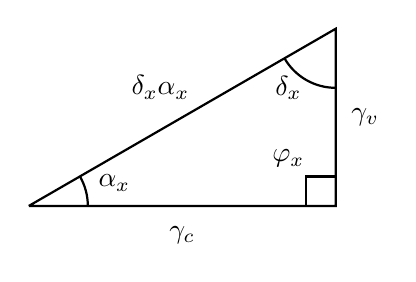
\begin{tikzpicture}[scale=1.5]
    \draw[thick] (0,0)--({3*sqrt(3)/2},0)--({3*sqrt(3)/2},1.5)--(0,0);
    \draw[thick] (0.5,0) arc [start angle=0, delta angle=30, radius=0.5];
    \draw[thick] ({3*sqrt(3)/2},1) arc [start angle=-90, delta angle=-60, radius=0.5];
    \draw[thick] ({3*sqrt(3)/2-0.25},0)--({3*sqrt(3)/2-0.25},0.25)--({3*sqrt(3)/2},0.25);
    \node at ({3*sqrt(3)/4},-0.25) {$\gamma_c$};
    \node at ({3*sqrt(3)/2+0.25}, 0.75) {$\gamma_v$};
    \node at (42:1.5) {$\delta_x\alpha_x$};
    \node at (15:0.75) {$\alpha_x$};
    \node at ({3*sqrt(3)/2-0.4},0.4) {$\varphi_x$};
    \node at ({3*sqrt(3)/2-0.4},1) {$\delta_x$};
\end{tikzpicture}\\
\noindent In terms of our general axis vantage tilt angles, the law of sines produces the resulting relationship:
\begin{flalign*}
&\frac{\gamma_v}{\sin\alpha_x}=\frac{\gamma_c}{\sin\delta_x}=\frac{1}{\beta_v\beta_c\sin(\pi - (\alpha_x+\delta_x))}
=\frac{\alpha_x\delta_x}{\sin\varphi}&&
\end{flalign*}

\subsubsection*{Metric:}
\noindent The seven dimensional positive definite metric interval in plain form with natural units is:
\begin{flalign*}
ds^2=&d\tau^2 + dx_t^2 + dt_x^2 + dy_t^2 + dt_y^2 + dz_t^2 + dt_x^2 = d\tau^2 + \sum_i(di_t^2 + dt_i^2), i \in x, y, z&&
\end{flalign*}
\noindent Accounting for relativistic distortions, we find the full form works out to:
\begin{flalign*}
ds^2=&d\tau^2 + \sum_i(\frac{c_i^2}{c^4}di_t^2 + \frac{v_i^2}{c^2}dt_i^2)=d\tau^2 + \sum_i\frac{v_i^2}{c^2}dt_i + \frac{1}{c^2}\sum_i\frac{c_i^2}{c^2}di_t=d\tau^2 + \sum_i\frac{1}{\alpha_i^2}dt_i + \frac{1}{c^2}\sum_i\frac{1}{\delta_i^2}di_t&&\\
&=g_{ij}dx^idx^j&&\\
&\quad\text{where}\quad g_{ij}=
\begin{pmatrix}
1& & & & & & \\
& \frac{1}{\alpha_x}& & & & & \\
& & \frac{1}{c^2\delta_x}& & & & \\
& & & \frac{1}{\alpha_y}& & & \\
& & & & \frac{1}{c^2\delta_y}& & \\
& & & & & \frac{1}{\alpha_z}& \\
& & & & & & \frac{1}{c^2\delta_z}\\
\end{pmatrix}&&
\end{flalign*}
\noindent Now to scale, it makes sense to choose an interval unit that is faithful to the dual conjugate nature of [m] and [s], which we choose tentatively, to be [ms]. What this entails is scaling the interval elements by $\sqrt{c}^2$, as appropriate per dimensionality, like so:
\begin{flalign*}
ds^2=&c d\tau^2 + \sum_i\left(\frac{1}{c} di_t^2 + c dt_i^2\right)&&\\
\end{flalign*}
\noindent And since the R7 space is rotational purely, we include the tilt angles that scale space according to observer-individual inter-action dynamics. Either squared according to metric interval elements, or not squared according to light and the postulate that all observers and individuals in the overall R7 space follow null geodesics at the speed of light $c$:
\begin{flalign*}
ds^2 =&\frac{c_\tau^2}{c^2}c d\tau^2 + \sum_i\left(\frac{c_i^2}{c^2}\frac{1}{c}  di_t^2 + \frac{v_i^2}{c^2} c dt_i^2\right) = c\beta_\tau^2 d\tau^2 + \sum_i \left( \frac{1}{c}\beta_c^2 di_t^2 + c\beta_v^2 dt_i^2\right) = \frac{c}{\Pi^2} d\tau^2 + \sum_i \left(\frac{1}{c\delta_i^2} di_t^2 + \frac{c}{\alpha_i^2} dt_i^2 \right)&&\\
&\text{or alternatively, TBD, un-squared tilt scaling} =\frac{c}{\Pi} d\tau^2 + \sum_i \left(\frac{1}{c\delta_i} di_t^2 + \frac{c}{\alpha_i} dt_i^2 \right)
\end{flalign*}
\noindent Note, $\Pi$ is a variation of the alternating Heaviside, a yet to be determined stroboscopic `tick-tock` universal time phase function that tau alternates between to mediate the spacetime-timespace inter-actions that forms the basis for the Cross Product Interaction Mechanism and universal action minimization.


\begin{itemize}
\item[.]
\end{itemize}


\noindent The reason for this updated choice is that \(\alpha_x\) represents the "occupant vantage tilt" between reference frames for individuals and observers in our higher-dimensional \(\mathbb{R}^7\) space, where:

\begin{itemize}
    \item[\textbf{.}] The adjacent side of length \(1\) represents the rest frame;
    \item[\textbf{.}] The opposite side of length \(\beta_v \Gamma_x\) represents the velocity-dependent distortion;
    \item[\textbf{.}] The hypotenuse of length \(\Gamma_x\) represents the relativistic distortion factor (here, the temporal).
\end{itemize}

\noindent This geometric representation enables one to replace hyperbolic functions in Minkowski space with simple Euclidean rotations in the extended 7-dimensional space, making relativistic transformations more intuitively accessible, while preserving their standard mathematical structure.\\

\noindent This choice will be demonstrated by applying the 7-lifts to the standard \(x\) and \(x'\) dimensional light-clock setup, then rotating to and from primed and unprimed frames, and finally projecting back down to standard Minkowski spacetime, where the usual Lorentz transformations are recovered:

\begin{flalign*}
    &t' = \Gamma_x (t \pm \frac{v_x}{c^2}x) \\
    &x' = \Gamma_x (x \pm v_x t)
\end{flalign*}

\noindent (Sign depends on direction of motion between frames, chosen by convention.)\\

\noindent First, 7-lift \(k\) and \(k'\) to 7D space, frames \(K\) and \(K'\):

\begin{flalign*}
    K_{\{\tau, t_x, x_t\}}^{(t, x)} &=
    R_{\tau t_x}^{(+\alpha_x)} k_{\{t, x\}}^{(v)} =
    \begin{pmatrix}
        \cos\alpha_x & \sin\alpha_x & 0\\
        -\sin\alpha_x & \cos\alpha_x & 0\\
        0 & 0 & 1
    \end{pmatrix}
    \begin{pmatrix}
        t \\
        A \\
        x
    \end{pmatrix} \\
    &= \begin{pmatrix}
        t\cos\alpha_x + A\sin\alpha_x \\
        A\cos\alpha_x - t\sin\alpha_x \\
        x
    \end{pmatrix}
\end{flalign*}

\begin{flalign*}
    {K'}_{\{\tau', t_x', x_t'\}}^{(t', x')} &=
    R_{\tau t_x}^{(-\alpha_x)} {k'}_{\{t', x'\}}^{(v')} =
    \begin{pmatrix}
        \cos\alpha_x & -\sin\alpha_x & 0\\
        \sin\alpha_x & \cos\alpha_x & 0\\
        0 & 0 & 1
    \end{pmatrix}
    \begin{pmatrix}
        t' \\
        A' \\
        x'
    \end{pmatrix} \\
    &= \begin{pmatrix}
        t'\cos\alpha_x - A'\sin\alpha_x \\
        A'\cos\alpha_x + t'\sin\alpha_x \\
        x'
    \end{pmatrix}
\end{flalign*}

\noindent Next, rotate each lifted frame by double angle \(2\alpha_x\):

\begin{flalign*}
    K_{\{\tau', t_x', x_t'\}}^{*(t, x)} &=
    R_{\tau t_x}^{(-2\alpha_x)} K_{\{\tau, t_x, x_t\}}^{(t,x)} \\
    &= \begin{pmatrix}
        \cos 2\alpha_x & -\sin 2\alpha_x & 0\\
        \sin 2\alpha_x & \cos 2\alpha_x & 0\\
        0 & 0 & 1
    \end{pmatrix}
    \begin{pmatrix}
        \tau \\
        t_x \\
        x_t
    \end{pmatrix}
\end{flalign*}

\noindent Similarly,

\begin{flalign*}
    {K'}_{\{\tau, t_x, x_t\}}^{*(t', x')} &=
    R_{\tau t_x}^{(+2\alpha_x)} {K'}_{\{\tau', t_x', x_t'\}}^{(t', x')}
\end{flalign*}

\noindent Finally, squeeze each rotated star frame back down to 2D with tilt coefficient \(\lambda = \pm \beta_v \Gamma_x\):

\begin{flalign*}
    {k'}_{\{t', x'\}}^{(v)} &= \pi^-(+\alpha_x) K_{\{\tau', t_x', x_t'\}}^{*(t, x)} \\
    &= \begin{pmatrix}
        1 & \lambda & \frac{1}{c}\lambda \\
        1 & \lambda & c\lambda
    \end{pmatrix}
    \begin{pmatrix}
        \tau' \\
        t_x' \\
        x_t'
    \end{pmatrix} \\
    &= \Gamma_x (t + \frac{v_x}{c^2} x,\, x + v_x t)
\end{flalign*}

\begin{flalign*}
    k_{\{t, x\}}^{(v)} &= {\pi}^-(-\alpha_x) {K'}_{\{\tau, t_x, x_t\}}^{*(t', x')} \\
    &= \begin{pmatrix}
        1 & \lambda & \frac{1}{c}\lambda \\
        1 & \lambda & c\lambda
    \end{pmatrix}
    \begin{pmatrix}
        \tau \\
        t_x \\
        x_t
    \end{pmatrix} \\
    &= \Gamma_x (t' - \frac{v_x}{c^2} x',\, x' - v_x t')
\end{flalign*}

\noindent Thus, the standard Lorentz transformations are recovered **exactly**, but derived from positive-definite rotational dynamics in \(\mathbb{R}^7\), using the new \(\Gamma_x\) unified triangle structure.




TIME MACHINE FOR PEACE SOCIAL INVENTION PROGRAM
\end{document}